\documentclass{article}
\usepackage{fancyhdr}
\usepackage{ctex}
\usepackage{listings}
\usepackage{graphicx}
\usepackage[a4paper, body={18cm,22cm}]{geometry}
\usepackage{amsmath,amssymb,amstext,wasysym,enumerate,graphicx}
\usepackage{float,abstract,booktabs,indentfirst,amsmath}
\usepackage{array}
\usepackage{booktabs}
\usepackage{multirow}
\usepackage{url}
\usepackage{diagbox}
\usepackage{hyperref}
\usepackage{listings}
\renewcommand\arraystretch{1.4}
\usepackage{indentfirst}
\setlength{\parindent}{2em}
\usepackage{enumitem}
\usepackage{accsupp}
\setmonofont{Consolas}
\usepackage{listings}
\usepackage{xcolor}
\usepackage{makecell}
\setCJKmonofont{黑体}
\newcommand\emptyaccsupp[1]{\BeginAccSupp{ActualText={}}#1\EndAccSupp{}}
\lstset{
    % language = C,
    xleftmargin = 3em,xrightmargin = 3em, aboveskip = 1em,
	backgroundcolor = \color{white}, % 背景色
	basicstyle = \small\ttfamily, % 基本样式 + 小号字体
	rulesepcolor= \color{gray}, % 代码块边框颜色
	breaklines = true, % 代码过长则换行
	numbers = left, % 行号在左侧显示
	numberstyle=\emptyaccsupp,
    numbersep = 14pt, 
    keywordstyle=\color{purple}\bfseries, % 关键字颜色
    commentstyle =\color{red!50!green!50!blue!60}, % 注释颜色
    stringstyle = \color{red}, % 字符串颜色
    morekeywords={ASSERT, int64_t, uint32_t},
	% frame = shadowbox, % 用(带影子效果)方框框住代码块
	frame = single, % 用(带影子效果)方框框住代码块
	showspaces = false, % 不显示空格
	columns = fixed, % 字间距固定
  framesep=1em
} 
\lstset{
    sensitive=true,
    moreemph={ASSERT, NULL}, emphstyle=\color{red}\bfseries,
    moreemph=[2]{int64_t, uint32_t, tid_t, uint8_t, int16_t, uint16_t, int32_t, size_t}, emphstyle=[2]\color{purple}\bfseries,
    }
%--------------------页眉--------------------%
\pagestyle{fancy}
\fancyhead[L]{}
\fancyhead[R]{}
\fancyhead[C]{《数据库系统及应用实践》课程实验报告}
\fancyfoot[C]{-\thepage-}
\renewcommand{\headrulewidth}{1.5pt}
%--------------------标题--------------------%
\begin{document}
\begin{center}
  \LARGE{{\textbf{\heiti 《数据库系统及应用实践》课程实验报告}}}

  \vspace{0.5em}

  \large 实验2:\texttt{SQL}练习
  \begin{table}[H]
    \centering
    \begin{tabular}{p{2cm}p{2cm}<{\centering}p{0.4cm}p{2cm}p{3cm}<{\centering}p{0.4cm}p{2cm}p{3cm}<{\centering}}
      姓\qquad 名: & 李鹏达 & \quad & 学\qquad 号: & 10225101460 & \quad & 完成日期: & 2024年3月21日 \\ \cline{2-2} \cline{5-5} \cline{8-8}
    \end{tabular}
  \end{table}
\end{center}
% \rule{\textwidth}{1pt}
%--------------------正文--------------------%
\section{实验目标}
\begin{enumerate}[noitemsep]
  \item 学习和掌握 \texttt{MySQL} 数据库管理系统中\texttt{SQL}的基本语法
  \item 能够编写\texttt{SQL}语句完成指定的查询
\end{enumerate}

\section{实验过程记录}

\subsection{创建数据表并导入数据}

首先下载实验2中的两个\texttt{SQL}脚本文件 \texttt{DDL+drop.sql} 和 \texttt{ largeRelationsInsertFile.sql}

然后运行在实验一中创建的数据库实例,并启动其中的 \texttt{bash shell}

\begin{lstlisting}[language=bash]
sudo docker run --name dbcourse -v ./datadir:/var/lib/mysql -d -p 53306:3306 dbcourse:v1
sudo docker exec -it dbcourse bash
\end{lstlisting}

\begin{figure}[H]
\centering
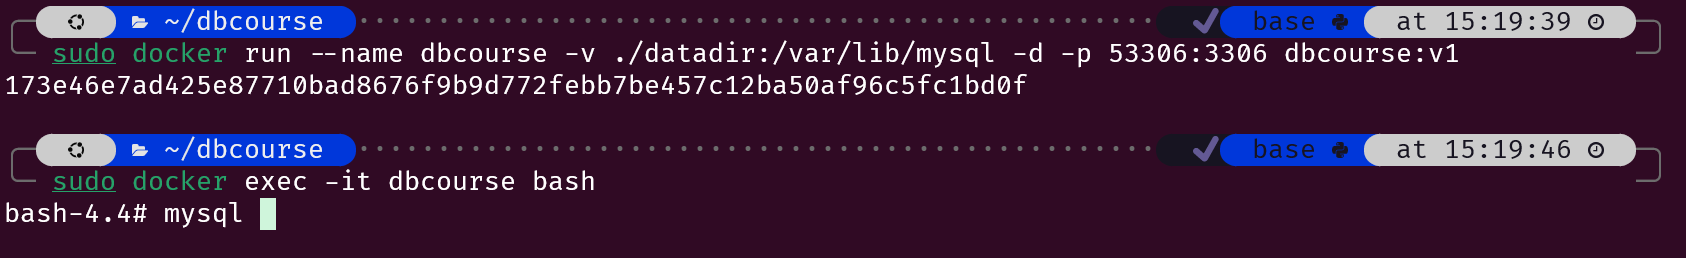
\includegraphics[width=0.9\textwidth]{img/1.png}
\caption{运行数据库实例并启动 \texttt{bash shell}}
\end{figure}

接着创建一个 \texttt{dbcourse} 文件夹,并 \texttt{cd} 到该文件夹下

\begin{lstlisting}[language=bash]
mkdir dbcourse
cd dbcourse
pwd
\end{lstlisting}

\begin{figure}[H]
\centering
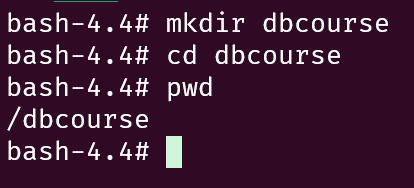
\includegraphics[width=0.4\textwidth]{img/2.png}
\caption{创建并进入文件夹}
\end{figure}

接着,在另一个终端中,将下载的两个 \texttt{SQL} 文件复制到容器内的\texttt{dbcourse} 文件夹下

\begin{lstlisting}[language=bash]
sudo docker cp ./DDL+drop.sql dbcourse:/dbcourse/
sudo docker cp ./largeRelationsInsertFile.sql.sql dbcourse:/dbcourse/
\end{lstlisting}

\begin{figure}[H]
\centering
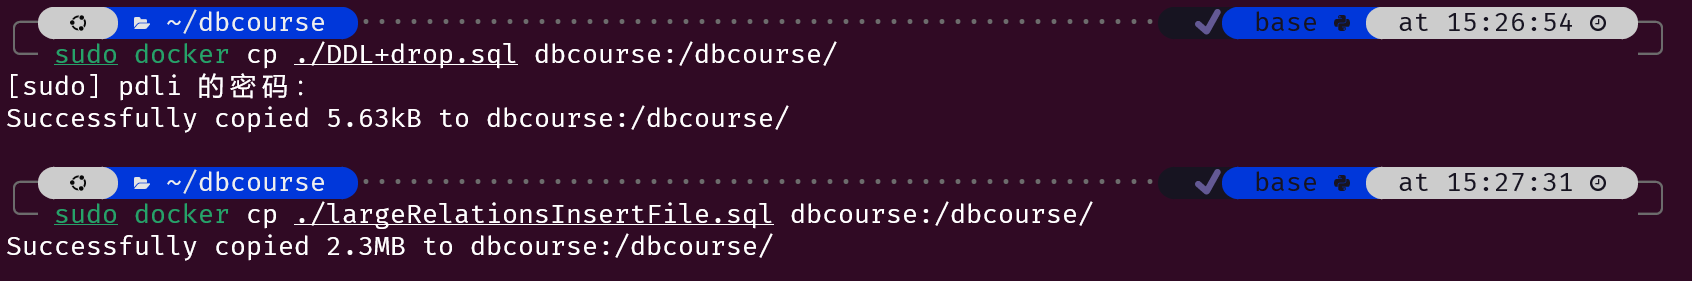
\includegraphics[width=0.9\textwidth]{img/3.png}
\caption{复制 \texttt{SQL} 文件到容器内}
\end{figure}

确认文件已经复制到容器内后,进入容器内的 \texttt{MySQL} 数据库

\begin{lstlisting}[language=bash]
ls -l
mysql -u root -p -D dbcourse
\end{lstlisting}

\begin{figure}[H]
\centering
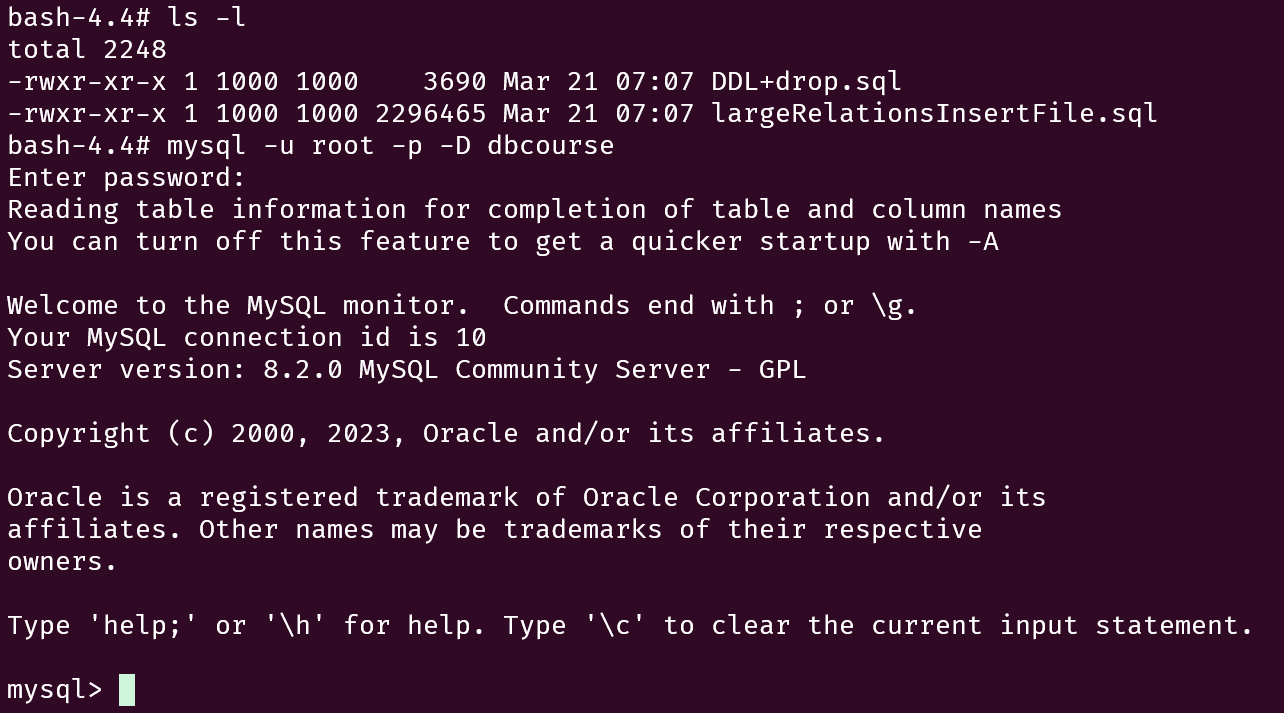
\includegraphics[width=0.6\textwidth]{img/4.png}
\caption{进入 \texttt{MySQL} 数据库}
\end{figure}

运行 \texttt{DDL+drop.sql} 文件,创建数据表,然后运行 \texttt{ largeRelationsInsertFile.sql} 文件,导入数据

\begin{lstlisting}[language=sql]
source DDL+drop.sql;
source largeRelationsInsertFile.sql;
\end{lstlisting}

\begin{figure}[H]
\centering
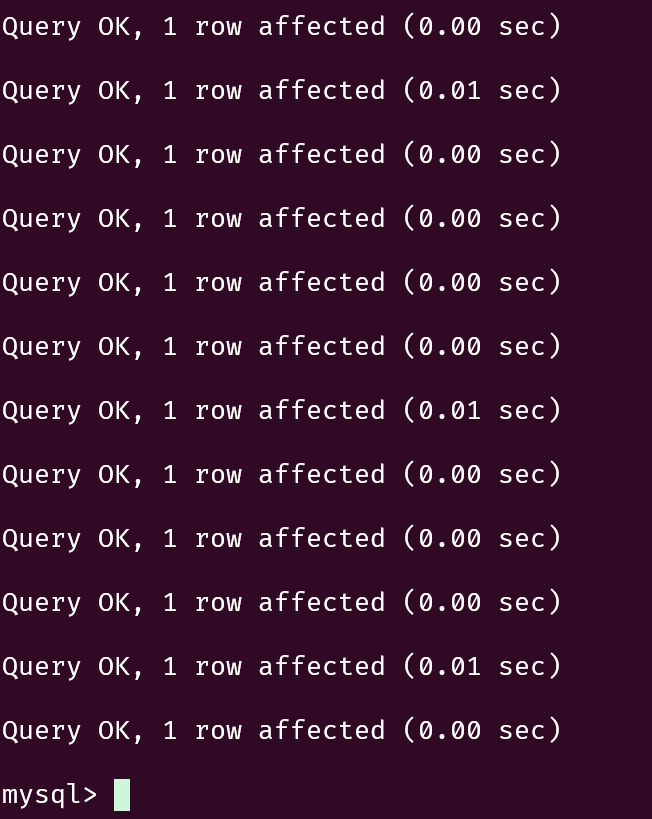
\includegraphics[width=0.5\textwidth]{img/5.png}
\caption{创建数据表并导入数据}
\end{figure}

执行下列 \texttt{SQL}语句,确认每张数据表中的记录数正确

\begin{lstlisting}[language=sql]
select count(*) from advisor;
select count(*) from classroom;
select count(*) from course;
select count(*) from department;
select count(*) from instructor;
select count(*) from prereq;
select count(*) from section;
select count(*) from student;
select count(*) from takes;
select count(*) from teaches;
select count(*) from time_slot;
\end{lstlisting}

结果为 2000,30,200,20,50,100,118,2000,30000,116,20,分别对应每张数据表中的记录数,说明数据表创建和数据导入成功。

使用 \texttt{exit} 命令退出 \texttt{MySQL} 数据库

\begin{lstlisting}[language=sql]
exit;
\end{lstlisting}

执行下列命令,通过 \texttt{MySQL}的命令行客户端执行单条\texttt{SQL}语句,并将查询结果保存到文件\texttt{department.csv}中

\begin{lstlisting}[language=bash]
mysql -u root -p -D dbcourse -e "select * from department;" > department.csv
cat department.csv
\end{lstlisting}

\begin{figure}[H]
\centering
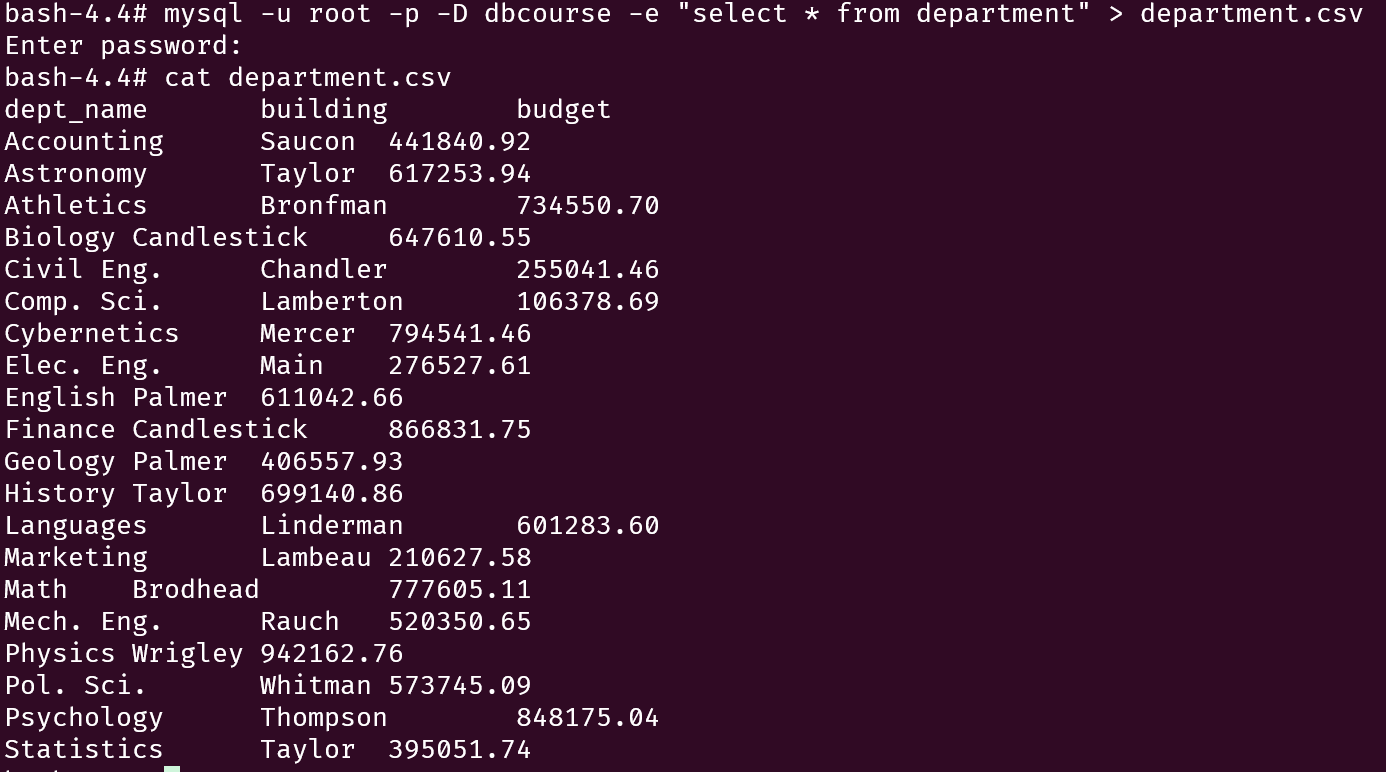
\includegraphics[width=0.9\textwidth]{img/6.png}
\caption{执行 \texttt{SQL} 语句并将结果保存到文件}
\end{figure}

\subsection{\texttt{SQL}练习}

\begin{enumerate}
  \item Find the names of all the instructors from Biology department.
  
\begin{lstlisting}[language=sql]
SELECT `name` FROM `instructor` WHERE `dept_name` = 'Biology';
\end{lstlisting}

结果如下:

\begin{figure}[H]
\centering
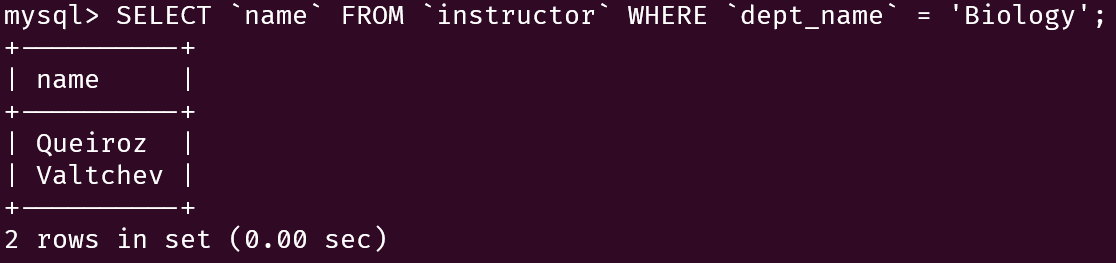
\includegraphics[width=0.9\textwidth]{img/7.png}
\caption{查询结果}
\end{figure}

\item Find the names of courses in Computer Science department which have 3 credits.
  
\begin{lstlisting}[language=sql]
SELECT `title` FROM `course` WHERE `dept_name` = 'Comp. Sci.' AND `credits` = 3;
\end{lstlisting}

结果如下:

\begin{figure}[H]
\centering
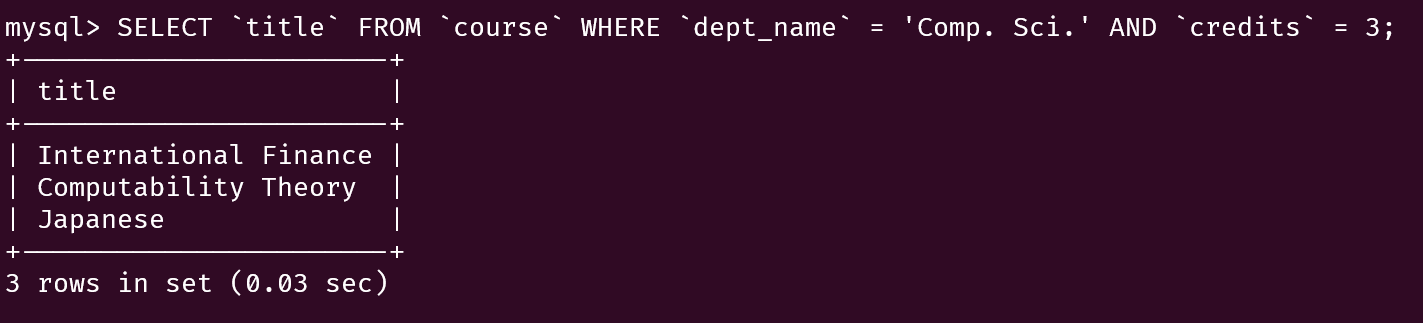
\includegraphics[width=0.9\textwidth]{img/8.png}
\caption{查询结果}
\end{figure}

\item For the student with ID 13403 (or any other value), show all course\_id and title of all courses taken by the student.

\begin{lstlisting}[language=sql]
SELECT `course_id`, `title` FROM `takes` NATURAL JOIN `course` WHERE `ID` = 13403;
\end{lstlisting}

结果如下:

\begin{figure}[H]
\centering
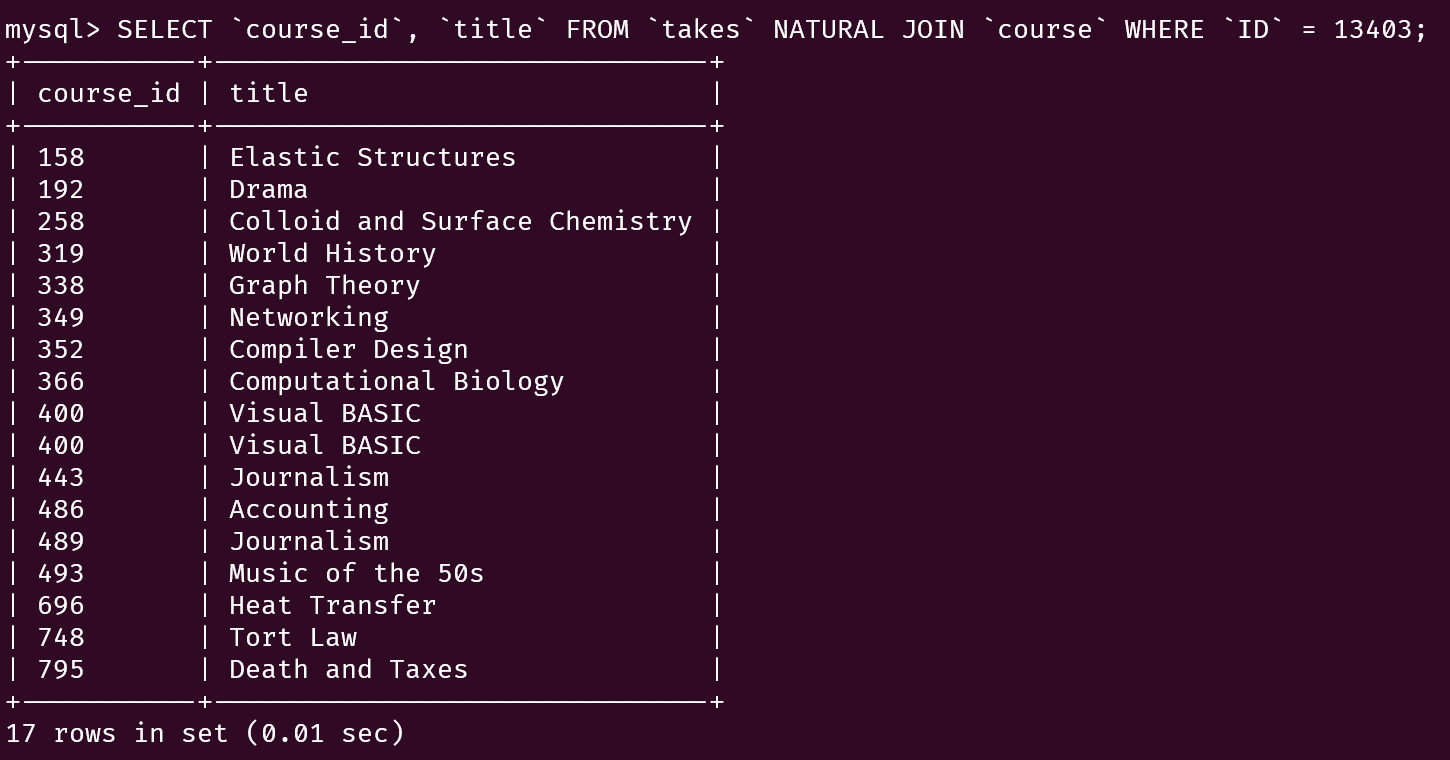
\includegraphics[width=0.9\textwidth]{img/9.png}
\caption{查询结果}
\end{figure}

\item As above, but show the total number of credits for such courses (taken by that student).

\begin{lstlisting}[language=sql]
SELECT `course_id`, `title`, `credits` FROM `takes` NATURAL JOIN `course` WHERE `ID` = 13403;
\end{lstlisting}

结果如下:

\begin{figure}[H]
\centering
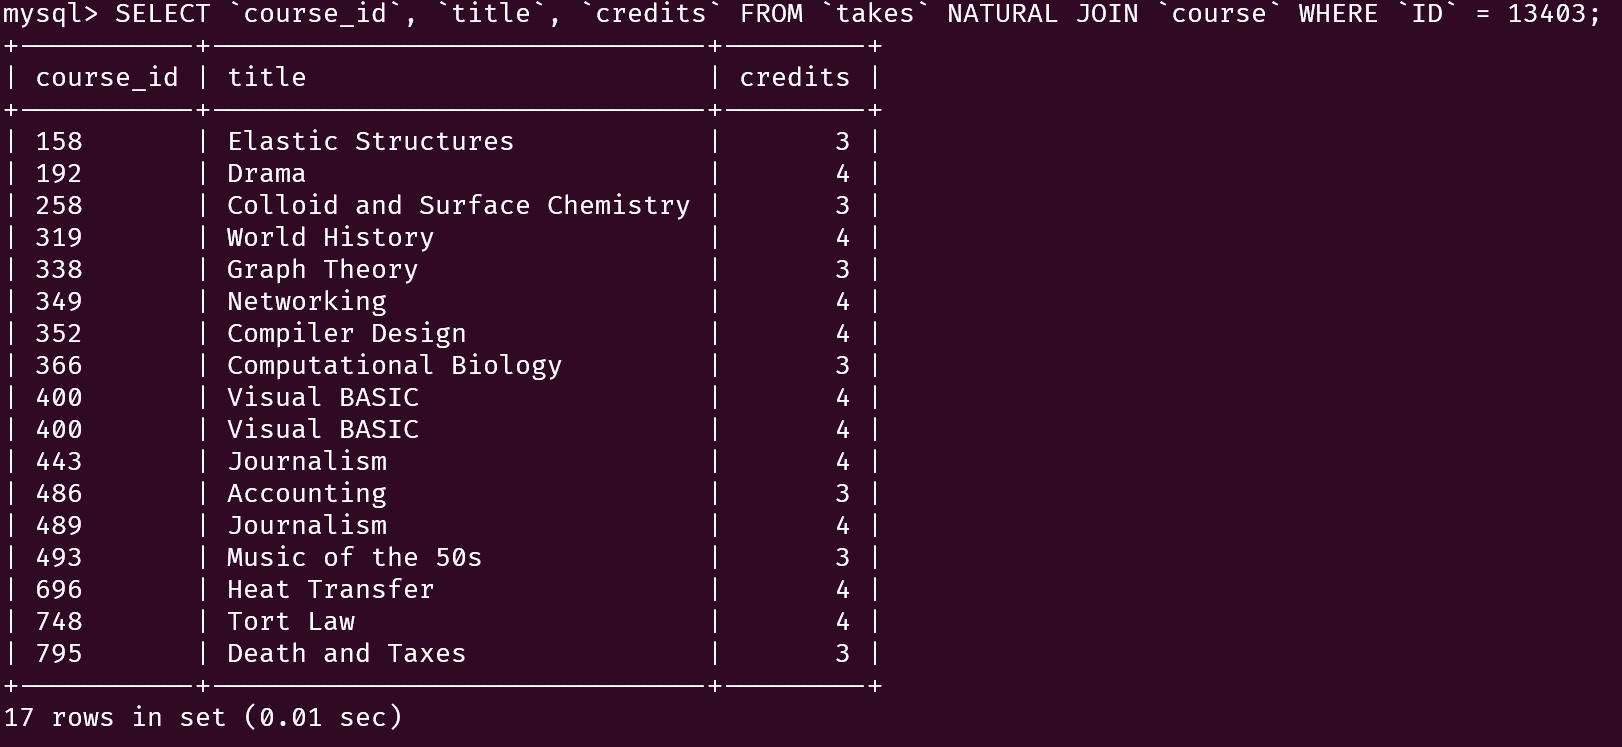
\includegraphics[width=0.7\textwidth]{img/10.png}
\caption{查询结果}
\end{figure}

\item Display the total credits for each of the students, along with the ID of the student.

\begin{lstlisting}[language=sql]
SELECT `ID`, SUM(`credits`) AS `total_credits` FROM `takes` NATURAL JOIN `course` GROUP BY `ID`;
\end{lstlisting}

结果如下:

\begin{figure}[H]
\centering
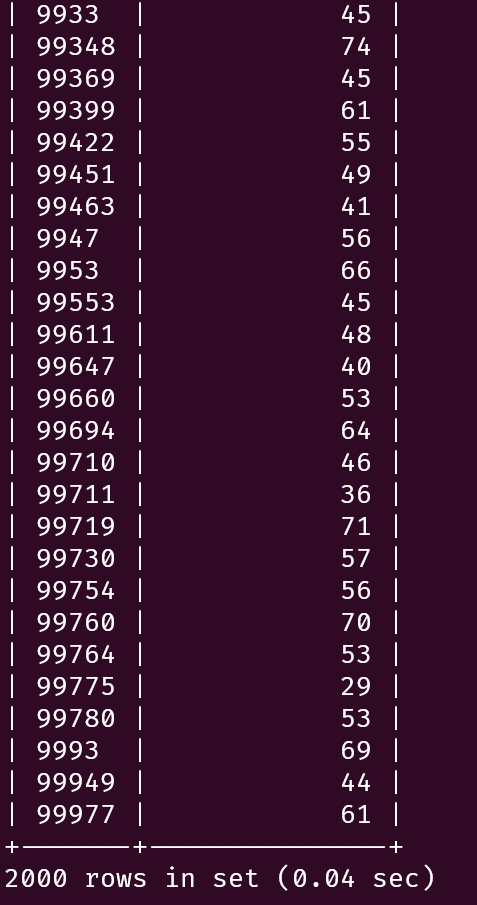
\includegraphics[width=0.4\textwidth]{img/11.png}
\caption{查询结果}
\end{figure}

\item Find the names of all students who have taken any Comp. Sci. course ever (there should be no duplicate names).

\begin{lstlisting}[language=sql]
SELECT DISTINCT `name` FROM `student` NATURAL JOIN `takes` NATURAL JOIN `course` WHERE `dept_name` = 'Comp. Sci.';
\end{lstlisting}

结果如下:

\begin{figure}[H] 
\centering
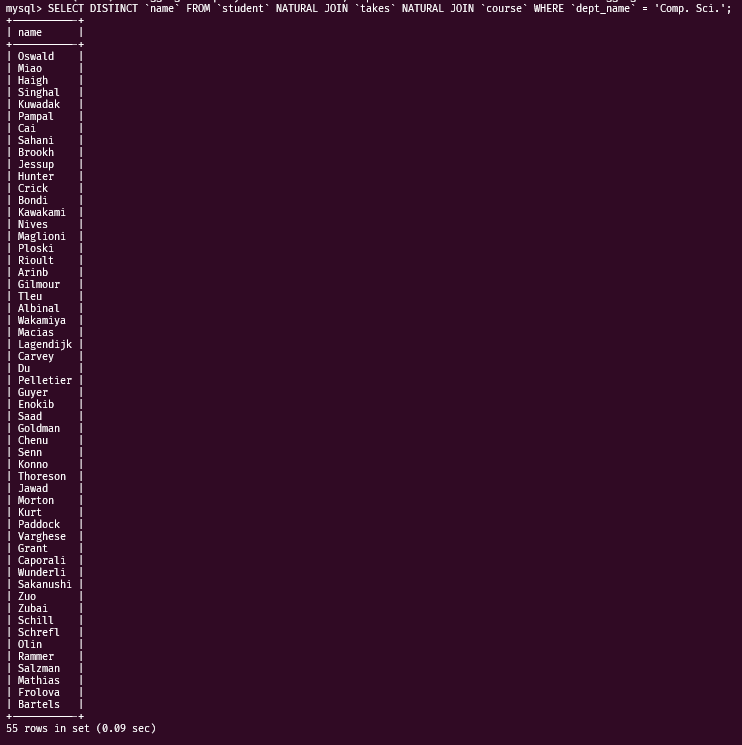
\includegraphics[width=0.9\textwidth]{img/12.png}
\caption{查询结果}
\end{figure}

\item Display the IDs of all instructors who have never taught a couse (interpret “taught” as “taught or is scheduled to teach”).

\begin{lstlisting}[language=sql]
SELECT `ID` FROM `instructor` NATURAL LEFT JOIN `teaches` WHERE `teaches`.`ID` IS NULL; 
\end{lstlisting}

结果如下:

\begin{figure}[H]
\centering
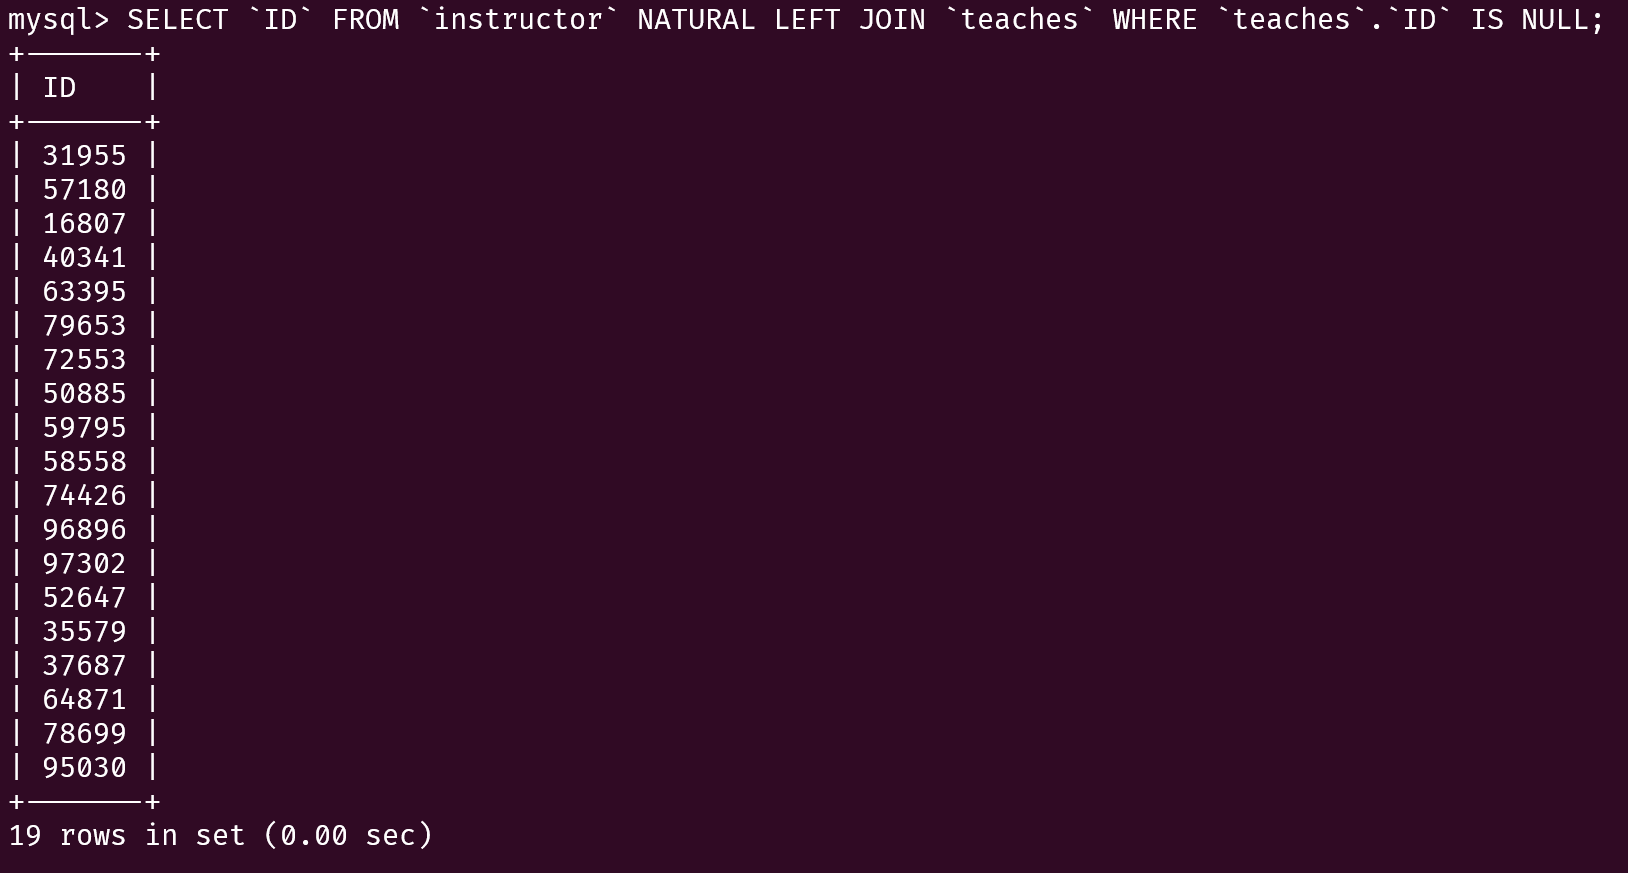
\includegraphics[width=0.9\textwidth]{img/13.png}
\caption{查询结果}
\end{figure}

\item As above, but display the names of the instructors also, not just the IDs.

\begin{lstlisting}[language=sql]
SELECT `ID`, `name` FROM `instructor` NATURAL LEFT JOIN `teaches` WHERE `teaches`.`ID` IS NULL;
\end{lstlisting}

结果如下:

\begin{figure}[H]
\centering
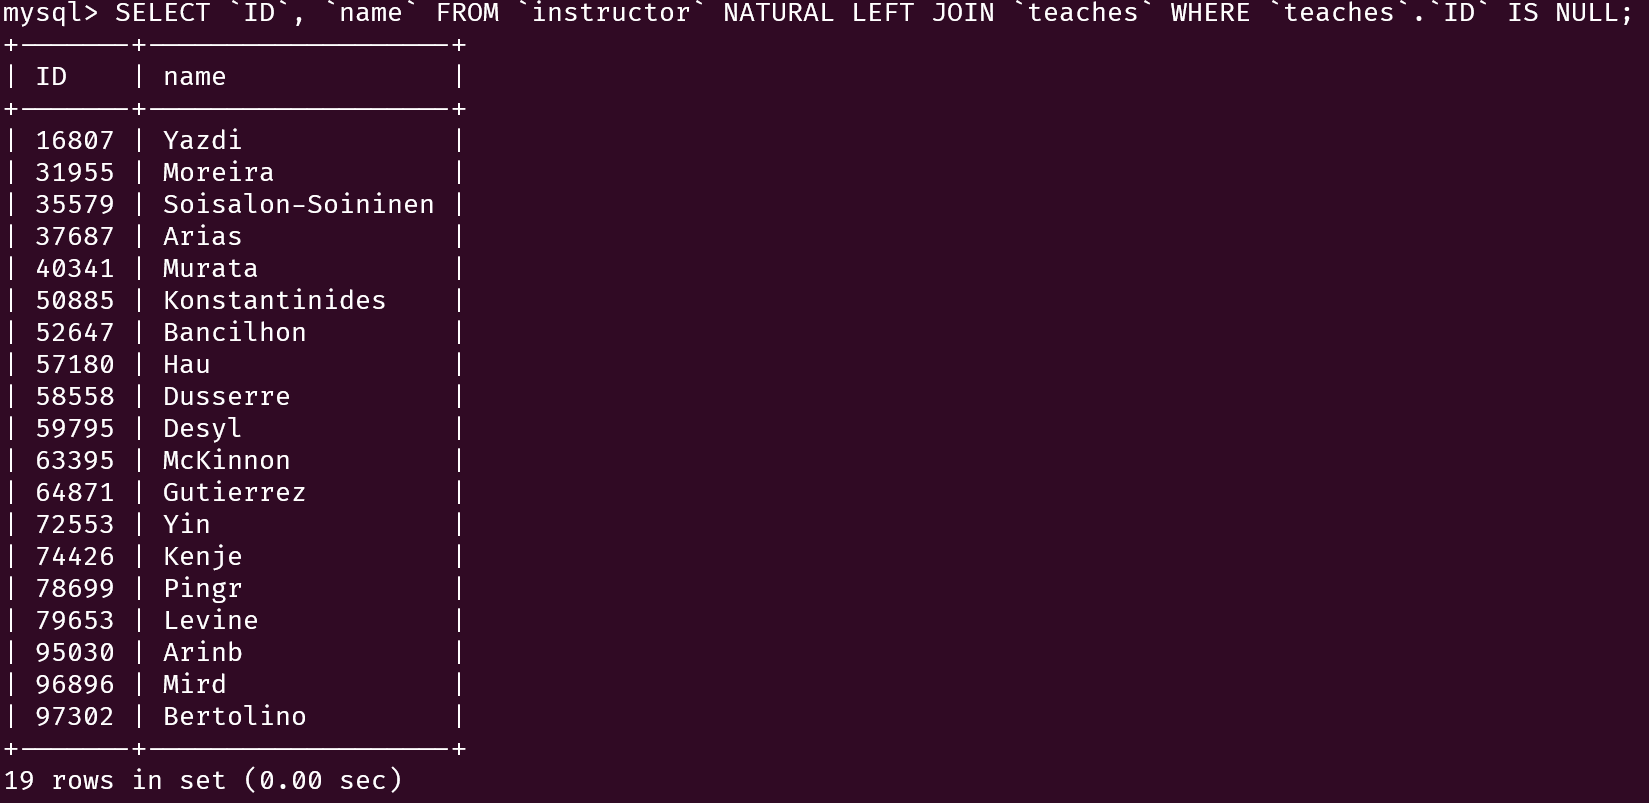
\includegraphics[height=7cm]{img/14.png} 
\caption{查询结果}
\end{figure}

\item You need to create a movie database. Create three tables, one for actors(AID, name), one for
movies(MID, title) and one for actor\_role(MID, AID, rolename). Use appropriate data types
for each of the attributes, and add appropriate primary/foreign key constraints.

\begin{lstlisting}[language=sql]
CREATE DATABASE `movie`;

CREATE TABLE `actors` (
  `AID` INT NOT NULL,
  `name` VARCHAR(50) NOT NULL,
  PRIMARY KEY (`AID`)
);

CREATE TABLE `movies` (
  `MID` INT NOT NULL,
  `title` VARCHAR(50) NOT NULL,
  PRIMARY KEY (`MID`)
);

CREATE TABLE `actor_role` (
  `MID` INT NOT NULL,
  `AID` INT NOT NULL,
  `rolename` VARCHAR(50) NOT NULL,
  PRIMARY KEY (`MID`, `AID`),
  FOREIGN KEY (`MID`) REFERENCES `movies`(`MID`),
  FOREIGN KEY (`AID`) REFERENCES `actors`(`AID`)
);
\end{lstlisting}

\begin{figure}[H]
\centering
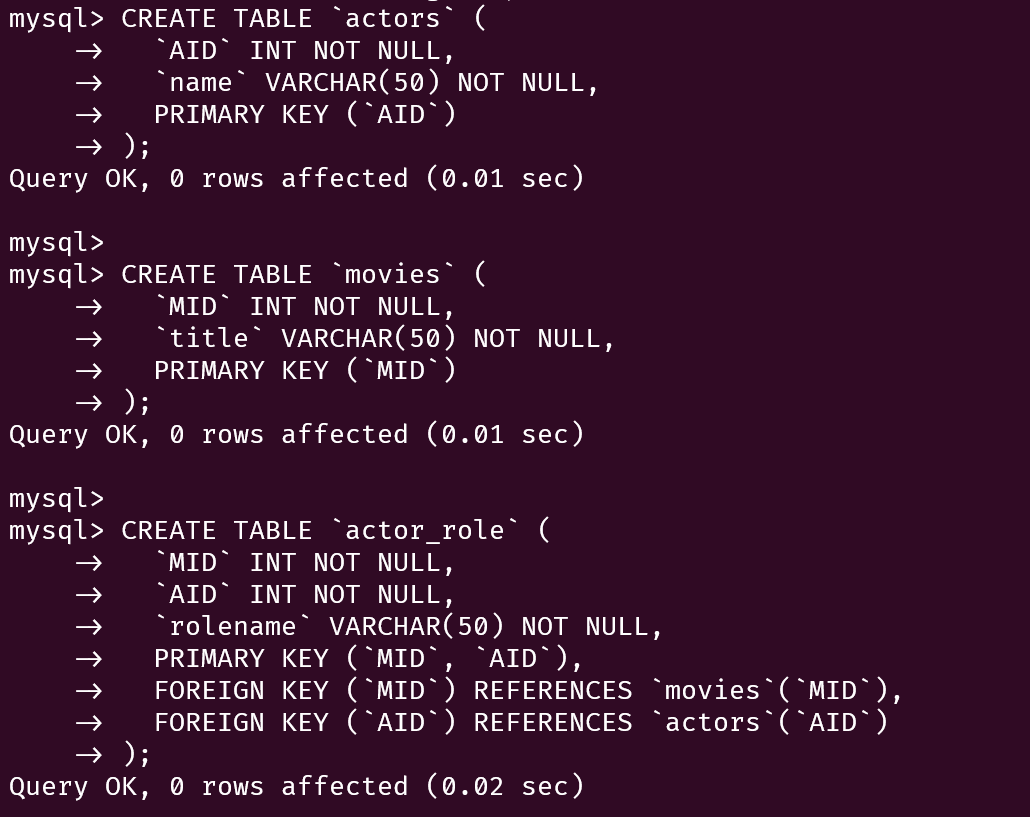
\includegraphics[width=0.42\textwidth]{img/15.png}
\caption{创建数据表}
\end{figure}

\item Insert data to the above tables (approx 3 to 6 rows in each table), including data for actor “Charlie Chaplin”, and for yourself (using your student number as ID).

\begin{lstlisting}[language=sql]
INSERT INTO `actors` (`AID`, `name`) VALUES (1, 'Charlie Chaplin'), (2, 'John Doe'), (460, 'Pengda Li');

INSERT INTO `movies` (`MID`, `title`) VALUES (1, 'The Great Dictator'), (2, 'Modern Times'), (3, 'City Lights');

INSERT INTO `actor_role` (`MID`, `AID`, `rolename`) VALUES (1, 1, 'Adenoid Hynkel'), (2, 1, 'The Tramp'), (3, 1, 'A Tramp'), (1, 2, 'Extra'), (2, 2, 'Extra'), (3, 460, 'Director');
\end{lstlisting}

\begin{figure}[H]
\centering
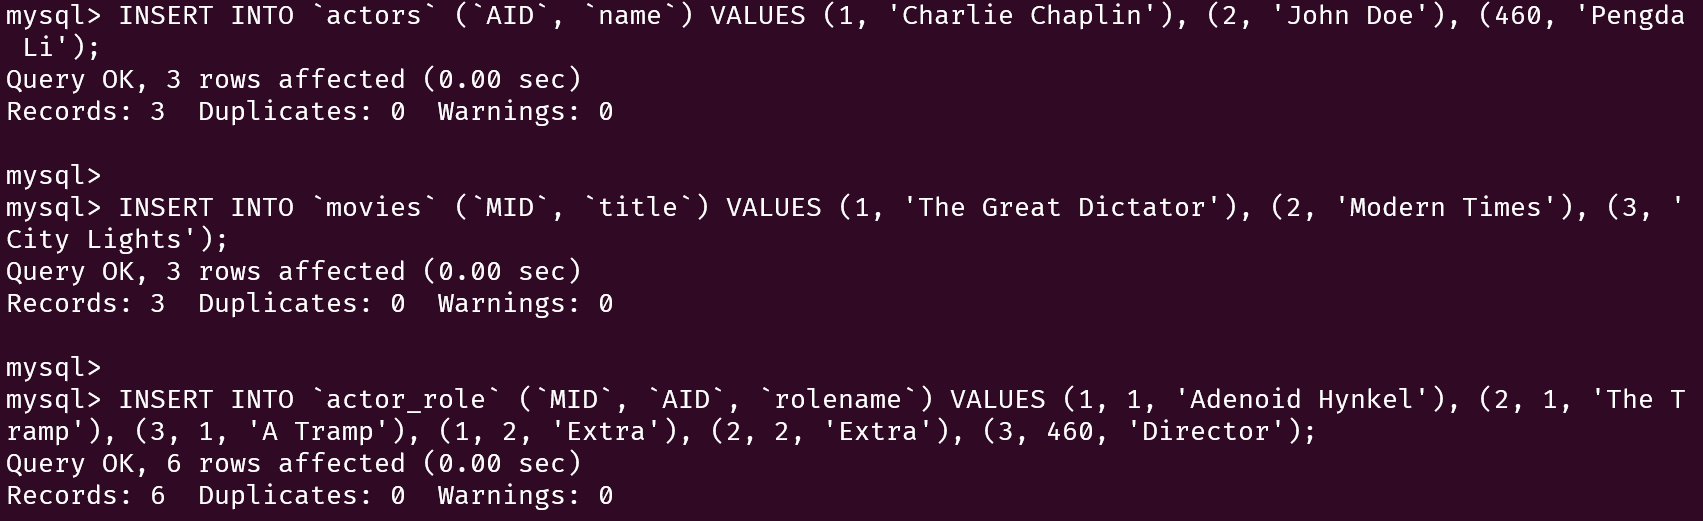
\includegraphics[width=0.9\textwidth]{img/16.png}
\caption{插入数据}
\end{figure}

\item Write a query to list all movies in which actor “Charlie Chaplin” has acted, along with the number of roles he had in that movie.

\begin{lstlisting}[language=sql]
SELECT `title`, COUNT(`rolename`) AS `roles` FROM `movies` NATURAL JOIN `actor_role` NATURAL JOIN `actors` WHERE `name` = 'Charlie Chaplin' GROUP BY `MID`;
\end{lstlisting}

结果如下:

\begin{figure}[H]
\centering
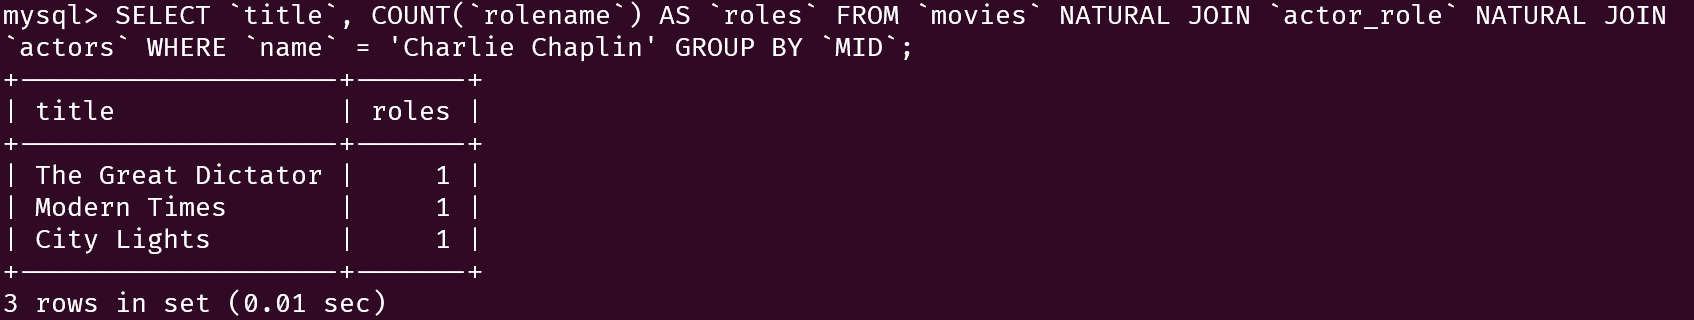
\includegraphics[width=0.9\textwidth]{img/17.png}
\caption{查询结果}
\end{figure}

\item Write a query to list the names of actors who have not acted in any movie.

\begin{lstlisting}[language=sql]
SELECT `name` FROM `actors` NATURAL LEFT JOIN `actor_role` WHERE `actor_role`.`MID` IS NULL;
\end{lstlisting}

结果如下:

\begin{figure}[H]
\centering
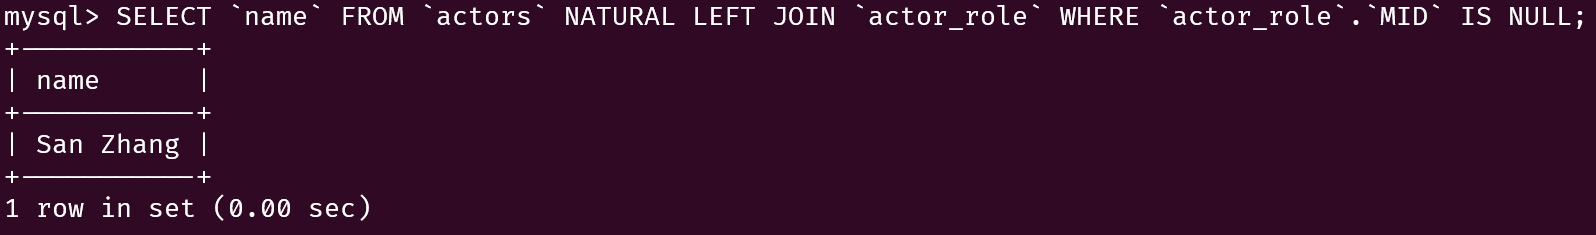
\includegraphics[width=0.9\textwidth]{img/18.png}
\caption{查询结果}
\end{figure}

\item List names of actors, along with titles of movies they have acted in. If they have not acted in any movie, show the movie title as null. (Do not use SQL outerjoin syntax here, write it from scratch.)

\begin{lstlisting}[language=sql]
SELECT `name`, `title` FROM `actors` NATURAL LEFT JOIN `actor_role` NATURAL LEFT JOIN `movies`;
\end{lstlisting}

结果如下:

\begin{figure}[H]
\centering
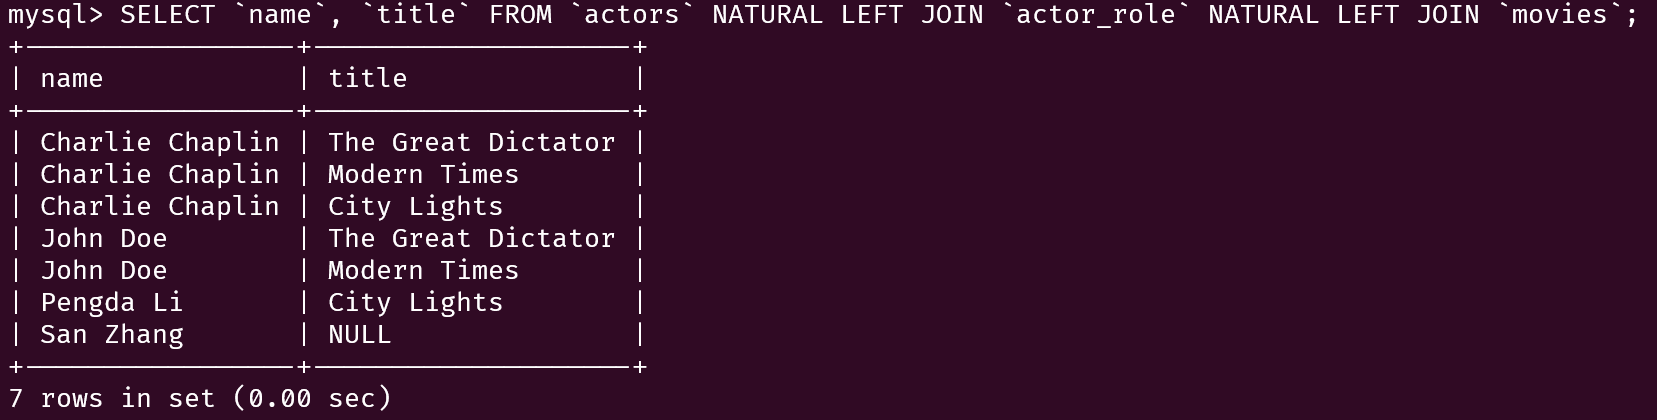
\includegraphics[width=0.9\textwidth]{img/19.png}
\caption{查询结果}
\end{figure}

\item Find the maximum and minimum enrollment across all sections, considering only sections that had some enrollment, don’t worry about those that had no students taking that section.

\begin{lstlisting}[language=sql]
WITH `enrollment` AS (
  SELECT `sec_id`, COUNT(`ID`) AS `enrollment` FROM `takes` GROUP BY `sec_id`
) SELECT MAX(`enrollment`) AS `max_enrollment`, MIN(`enrollment`) AS `min_enrollment` FROM `enrollment`;
\end{lstlisting}

结果如下:

\begin{figure}[H]
\centering
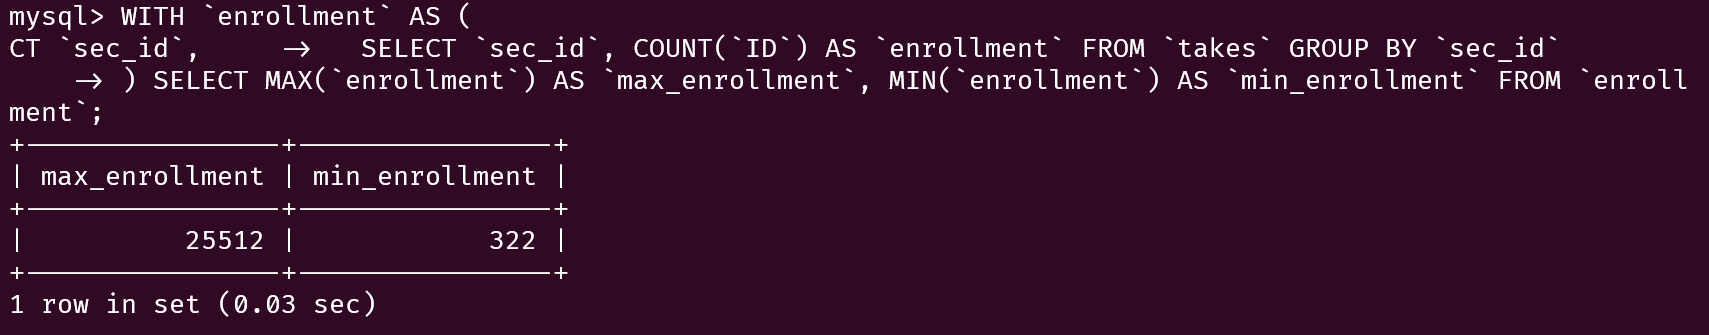
\includegraphics[width=0.9\textwidth]{img/20.png}
\caption{查询结果}
\end{figure}

\item Find all sections that had the maximum enrollment (along with the enrollment).

\begin{lstlisting}[language=sql]
WITH `enrollment` AS (
  SELECT `sec_id`, COUNT(`ID`) AS `enrollment` FROM `takes` GROUP BY `sec_id`
) SELECT `sec_id`, `enrollment` FROM `enrollment` WHERE `enrollment` = (SELECT MAX(`enrollment`) FROM `enrollment`);
\end{lstlisting}

\item As in step 14, but now it also includes sections with no students taking them; the enrollment for such sections should be treated as 0. Do this in two different ways.
\begin{itemize}
  \item Using a scalar subquery;
  \begin{lstlisting}[language=sql]
SELECT MAX(`enrollment`) AS `max_enrollment`, MIN(`enrollment`) AS `min_enrollment` FROM (SELECT `sec_id`, COALESCE((SELECT COUNT(`ID`) FROM `takes` WHERE `sec_id` = `section`.`sec_id`), 0) AS `enrollment` FROM `section`) AS `enrollments`;
  \end{lstlisting}

  结果如下:

  \begin{figure}[H]
  \centering
  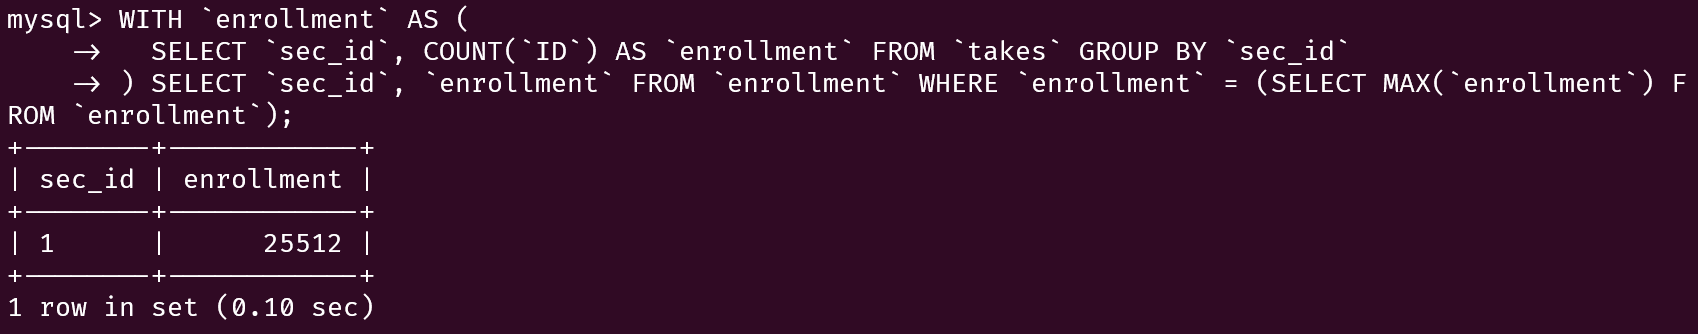
\includegraphics[width=0.9\textwidth]{img/21.png}
  \caption{查询结果}
  \end{figure}

  \item Using aggregation on a left outer join (use the SQL natural left outer join syntax);
  
  \begin{lstlisting}[language=sql]
SELECT MAX(`enrollment`) AS `max_enrollment`, MIN(`enrollment`) AS `min_enrollment` FROM (SELECT `sec_id`, COUNT(`ID`) AS `enrollment` FROM `section` NATURAL LEFT JOIN `takes` GROUP BY `sec_id`) AS `enrollments`;
  \end{lstlisting}

  结果如下:

  \begin{figure}[H]
  \centering
  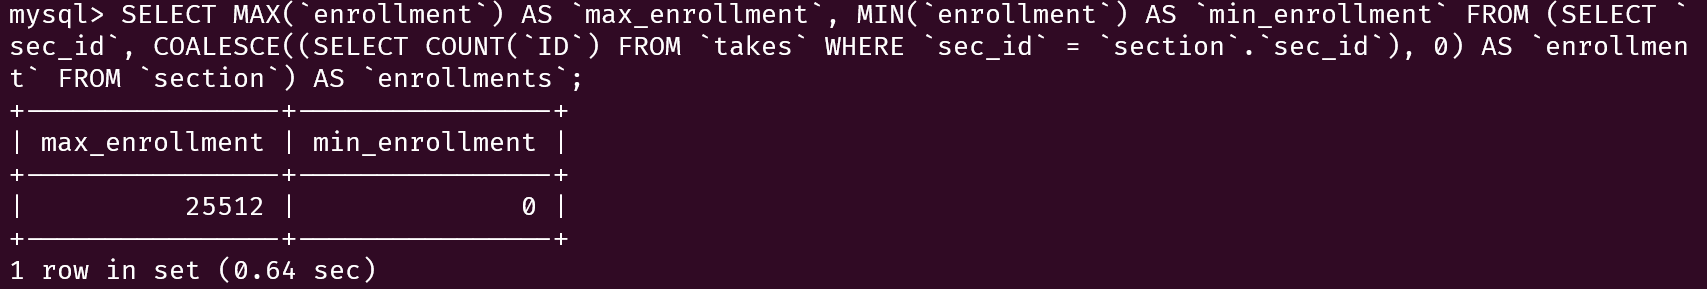
\includegraphics[width=0.9\textwidth]{img/22.png}
  \caption{查询结果}
  \end{figure}

\end{itemize}

\item Find all courses whose title starts with the string “Comp”.

\begin{lstlisting}[language=sql]
SELECT `title` FROM `course` WHERE `title` LIKE 'Comp%';
\end{lstlisting}

结果如下:

\begin{figure}[H]
\centering
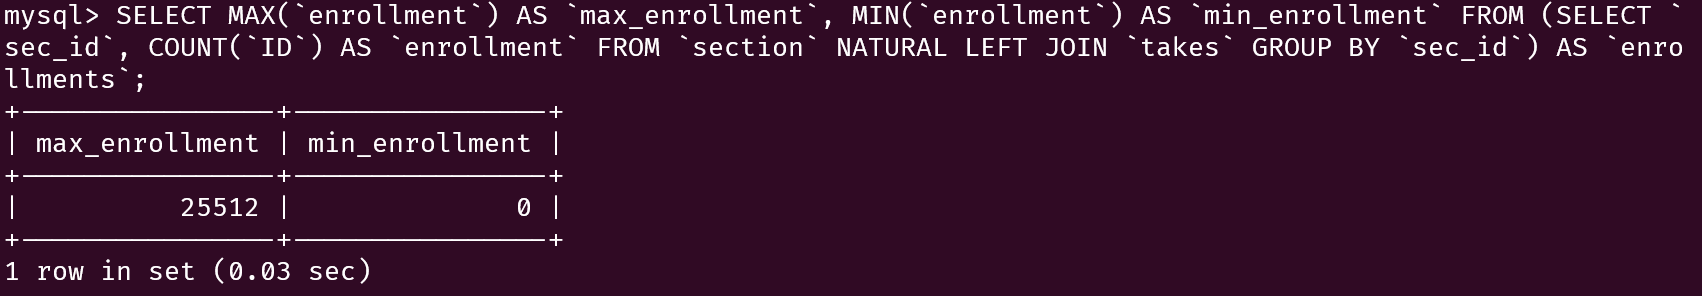
\includegraphics[width=0.9\textwidth]{img/23.png}
\caption{查询结果}
\end{figure}

\item Find instructors who have taught all courses in in Comp. Sci. Department.

\begin{itemize}
  \item Using the “not exists … except …” structure;
  \begin{lstlisting}[language=sql]
SELECT `ID`, `name` FROM `instructor` WHERE NOT EXISTS (SELECT `course_id` FROM `course` WHERE `dept_name` = 'Comp. Sci.' EXCEPT SELECT `course_id` FROM `teaches` WHERE `teaches`.`ID` = `instructor`.`ID`);
  \end{lstlisting}

  结果如下:

  \begin{figure}[H]
  \centering
  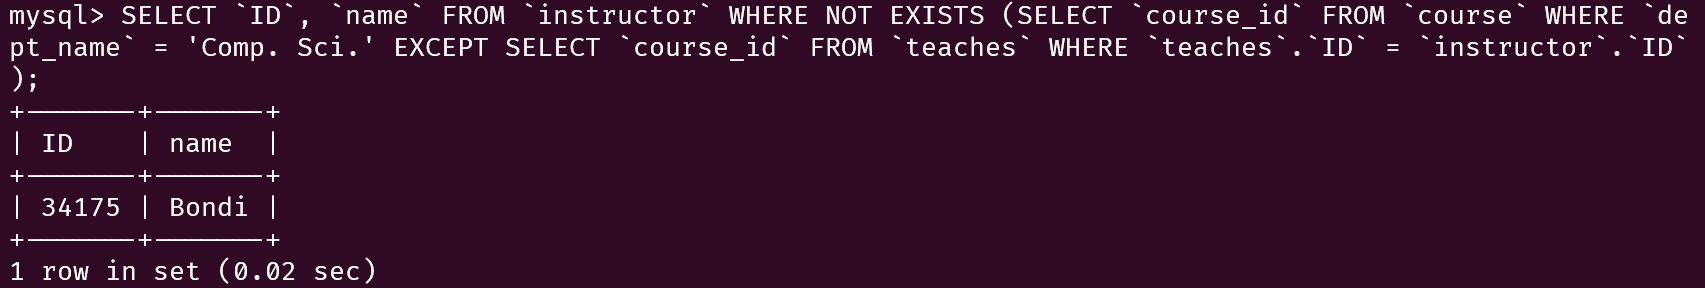
\includegraphics[width=0.9\textwidth]{img/25.png}
  \caption{查询结果}
  \end{figure}

  \item Using matching of counts (Don’t forget the distinct clause!).
  
  \begin{lstlisting}[language=sql]
SELECT `ID`, `name` FROM `instructor` WHERE (SELECT COUNT(DISTINCT `course_id`) FROM `course` WHERE `dept_name` = 'Comp. Sci.') = (SELECT COUNT(DISTINCT `course_id`) FROM `teaches` NATURAL JOIN `course` WHERE `teaches`.`ID` = `instructor`.`ID` AND `dept_name` = 'Comp. Sci.');
\end{lstlisting}

结果如下:

\begin{figure}[H]
\centering
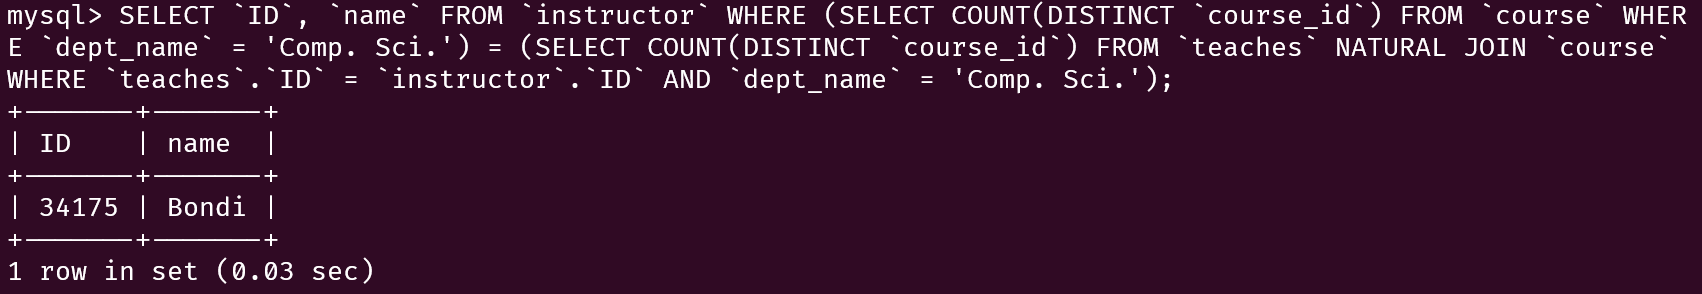
\includegraphics[width=0.9\textwidth]{img/26.png}
\caption{查询结果}
\end{figure}
\end{itemize}

\item Insert each instructor as a student, with tot\_cred = 0, in the same department.

\begin{lstlisting}[language=sql]
INSERT INTO `student` (`ID`, `name`, `dept_name`, `tot_cred`) SELECT `ID`, `name`, `dept_name`, 0 FROM `instructor`;
\end{lstlisting}

结果如下:

\begin{figure}[H]
\centering
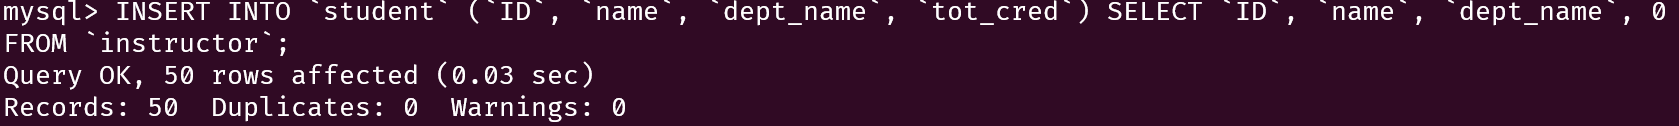
\includegraphics[width=0.9\textwidth]{img/27.png}
\caption{插入数据}
\end{figure}

\item Now delete all the newly added “students” above.

\begin{lstlisting}[language=sql]
DELETE FROM `student` WHERE `ID` IN (SELECT `ID` FROM `instructor`);
\end{lstlisting}

结果如下:

\begin{figure}[H]
\centering
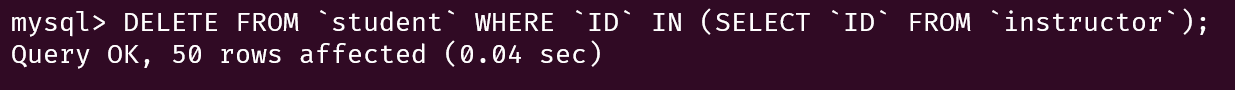
\includegraphics[width=0.9\textwidth]{img/28.png}
\caption{删除数据}
\end{figure}

\item Some of you may have noticed that the tot\_creds value for students did not match the credits from courses they have taken. Write and execute query to update tot\_creds based on the credits passed, to bring the database back to consistency.

\begin{lstlisting}[language=sql]
UPDATE `student` SET `tot_cred` = (SELECT SUM(`credits`) FROM `takes` NATURAL JOIN `course` WHERE `takes`.`ID` = `student`.`ID`);
\end{lstlisting}

结果如下:

\begin{figure}[H]
\centering
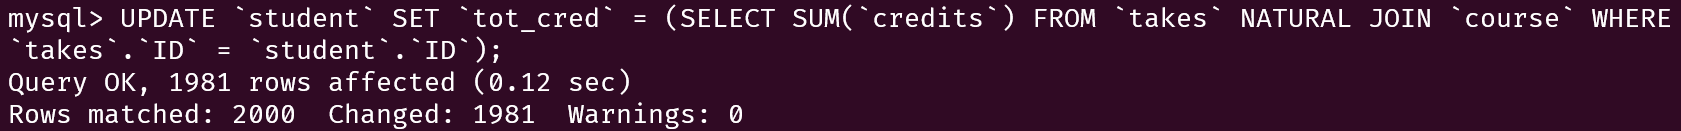
\includegraphics[width=0.9\textwidth]{img/29.png}
\caption{更新数据}
\end{figure}

\item Increase the salaries of instructors by 1000 times the number of course sections they have taught.

\begin{lstlisting}[language=sql]
UPDATE `instructor` SET `salary` = `salary` + 1000 * (SELECT COUNT(`sec_id`) FROM `teaches` WHERE `teaches`.`ID` = `instructor`.`ID`);
\end{lstlisting}

结果如下:

\begin{figure}[H]
\centering
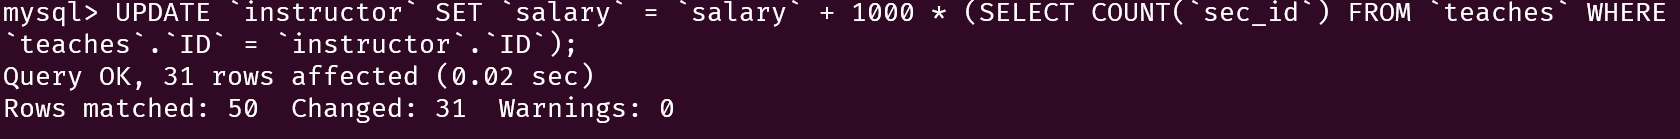
\includegraphics[width=0.9\textwidth]{img/30.png}
\caption{更新数据}
\end{figure}

\item The university rules allow an F grade to be overridden by any pass grade (A, A-, B+, B, B-, C+, C, C-, D, D-). Now, create a view that lists information about all fail grades that have not been overridden (the view should contain all attributes from the takes relation).

\begin{lstlisting}[language=sql]
CREATE VIEW `fail_grades` AS SELECT * FROM `takes` WHERE `grade` = 'F' AND NOT EXISTS (SELECT * FROM `takes` AS `override` WHERE `takes`.`ID` = `override`.`ID` AND `takes`.`course_id` = `override`.`course_id` AND `override`.`grade` IN ('A', 'A-', 'B+', 'B', 'B-', 'C+', 'C', 'C-', 'D', 'D-'));
\end{lstlisting}

结果如下:

\begin{figure}[H]
\centering

\includegraphics[width=0.9\textwidth]{img/31.png}
\caption{创建视图}
\end{figure}

\item Find all students who have 2 or more non-overridden F grades, and list them along with the F grades.

\begin{lstlisting}[language=sql]
SELECT `ID`, `course_id`, `grade` FROM `fail_grades` WHERE `ID` IN (SELECT `ID` FROM `fail_grades` GROUP BY `ID` HAVING COUNT(`grade`) >= 2);
\end{lstlisting}

结果如下:

\begin{figure}[H]
\centering
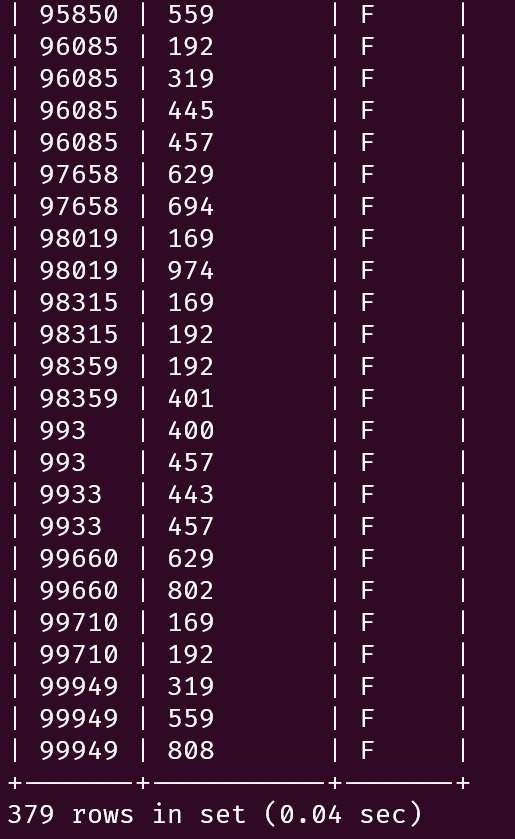
\includegraphics[width=0.3\textwidth]{img/32.png}
\caption{查询结果}
\end{figure}

\item Grades are mapped to a grade point as follows:

\begin{table}[h]
  \centering
  \begin{tabular}{|c|c|c|c|c|c|c|c|c|c|c|c|c|}
  \hline
  Grade & A+ & A & A- & B+ & B & B- & C+ & C & C- & D & D- & F \\
  \hline
  GP & 4.0 & 4.0 & 3.7 & 3.3 & 3.0 & 2.7 & 2.3 & 2.0 & 1.7 & 1.3 & 1.0 & 0.0 \\
  \hline
  \end{tabular}
  \caption{Grade to GP conversion}
  \label{tab:my_label}
  \end{table}
Create a table to store these mappings, and write a query to find the GPA (Grade Point Average) of each student, using this table. Make sure students who have not got a non-null grade in any course are displayed with a GPA of null.

\begin{lstlisting}[language=sql]
CREATE TABLE `grade_point` (
  `grade` CHAR(2) NOT NULL,
  `gp` DECIMAL(3, 1) NOT NULL,
  PRIMARY KEY (`grade`)
);

INSERT INTO `grade_point` (`grade`, `gp`) VALUES ('A+', 4.0), ('A', 4.0), ('A-', 3.7), ('B+', 3.3), ('B', 3.0), ('B-', 2.7), ('C+', 2.3), ('C', 2.0), ('C-', 1.5), ('D', 1.3), ('D-', 1.0), ('F', 0.0);

SELECT `ID`, SUM(`gp` * `credits`) / SUM(`credits`) AS `GPA` FROM `takes` NATURAL JOIN `grade_point` NATURAL JOIN `course` GROUP BY `ID`;
\end{lstlisting}

结果如下:

\begin{figure}[H]
\centering
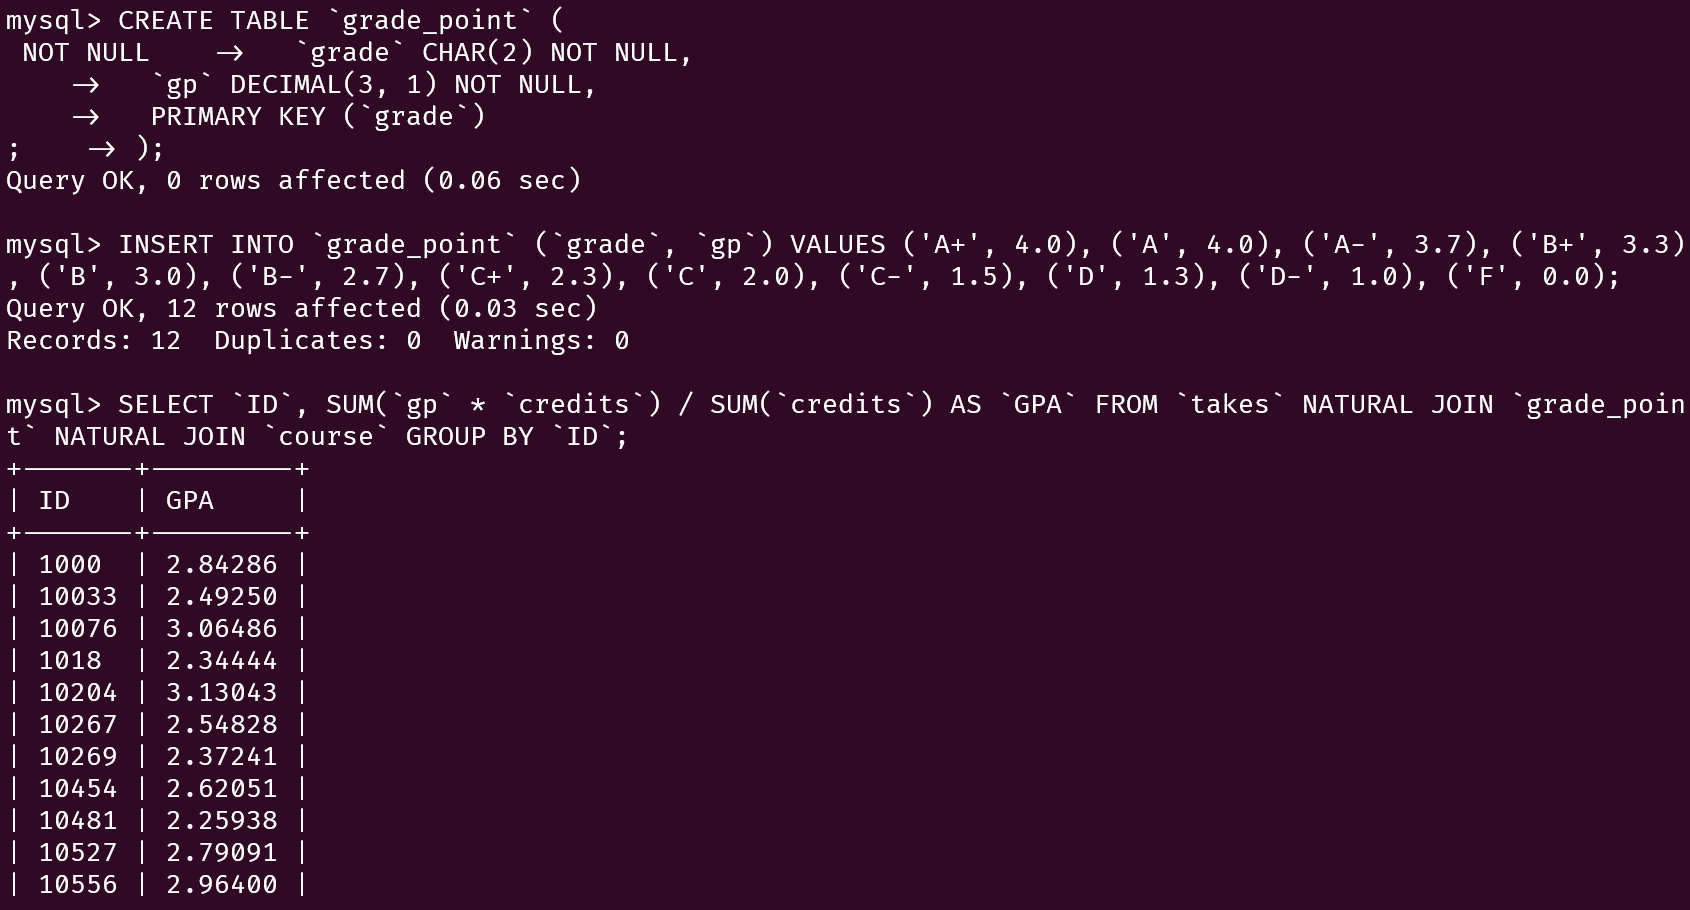
\includegraphics[width=0.8\textwidth]{img/33.png}
\caption{查询结果}
\end{figure}

\item Find all classrooms that have been assigned to more than one section at the same time. Display the rooms along with the assigned sections; Using a with clause or a view to simplify this query.

\begin{lstlisting}[language=sql]
WITH `conflict` AS (
  SELECT `room_number`, `time_slot_id` FROM `section` GROUP BY `room_number`, `time_slot_id` HAVING COUNT(`sec_id`) > 1
) SELECT `room_number`, `sec_id` FROM `section` WHERE `room_number` IN (SELECT `room_number` FROM `conflict`) AND `time_slot_id` IN (SELECT `time_slot_id` FROM `conflict`);
\end{lstlisting}

结果如下:

\begin{figure}[H]
\centering
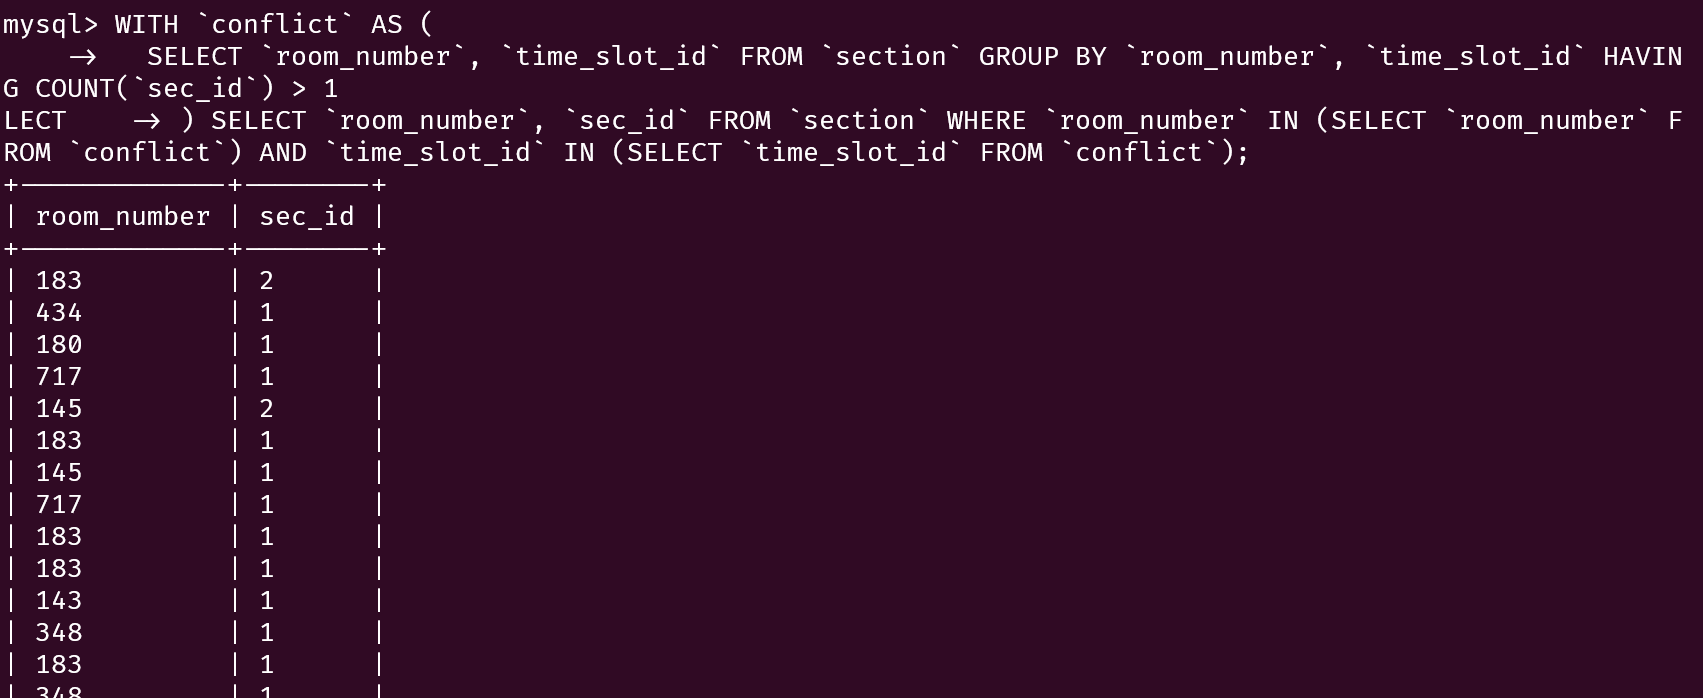
\includegraphics[width=0.9\textwidth]{img/34.png}
\caption{查询结果}
\end{figure}

\item Create a view faculty showing only the ID, name, and department of instructors.

\begin{lstlisting}[language=sql]
CREATE VIEW `faculty` AS SELECT `ID`, `name`, `dept_name` FROM `instructor`;
\end{lstlisting}

结果如下:

\begin{figure}[H]
\centering
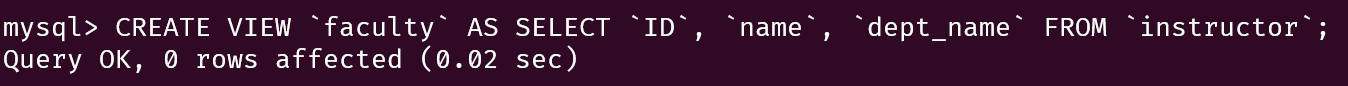
\includegraphics[width=0.9\textwidth]{img/35.png}
\caption{创建视图}
\end{figure}

\item Create a view CSinstructors, showing all information about instructors from the Comp. Sci. department.

\begin{lstlisting}[language=sql]
CREATE VIEW `CSinstructors` AS SELECT * FROM `instructor` WHERE `dept_name` = 'Comp. Sci.';
\end{lstlisting}

结果如下:

\begin{figure}[H]
\centering
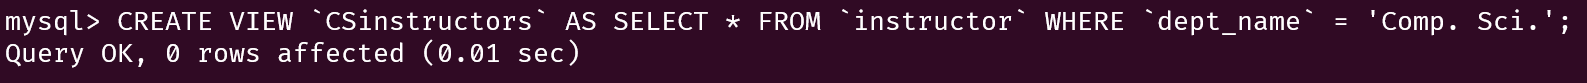
\includegraphics[width=0.9\textwidth]{img/36.png}
\caption{创建视图}
\end{figure}

\item Insert appropriate tuple into each of the views faculty and CSinstructors, to see what updates your database allows on views; explain what happens.

\begin{lstlisting}[language=sql]
INSERT INTO `faculty` (`ID`, `name`, `dept_name`) VALUES (10101, 'John Doe', 'Comp. Sci.');
INSERT INTO `CSinstructors` (`ID`, `name`, `dept_name`, `salary`) VALUES (10102, 'John Smith', 'Comp. Sci.', 100000);
\end{lstlisting}

结果如下:

\begin{figure}[H]
\centering
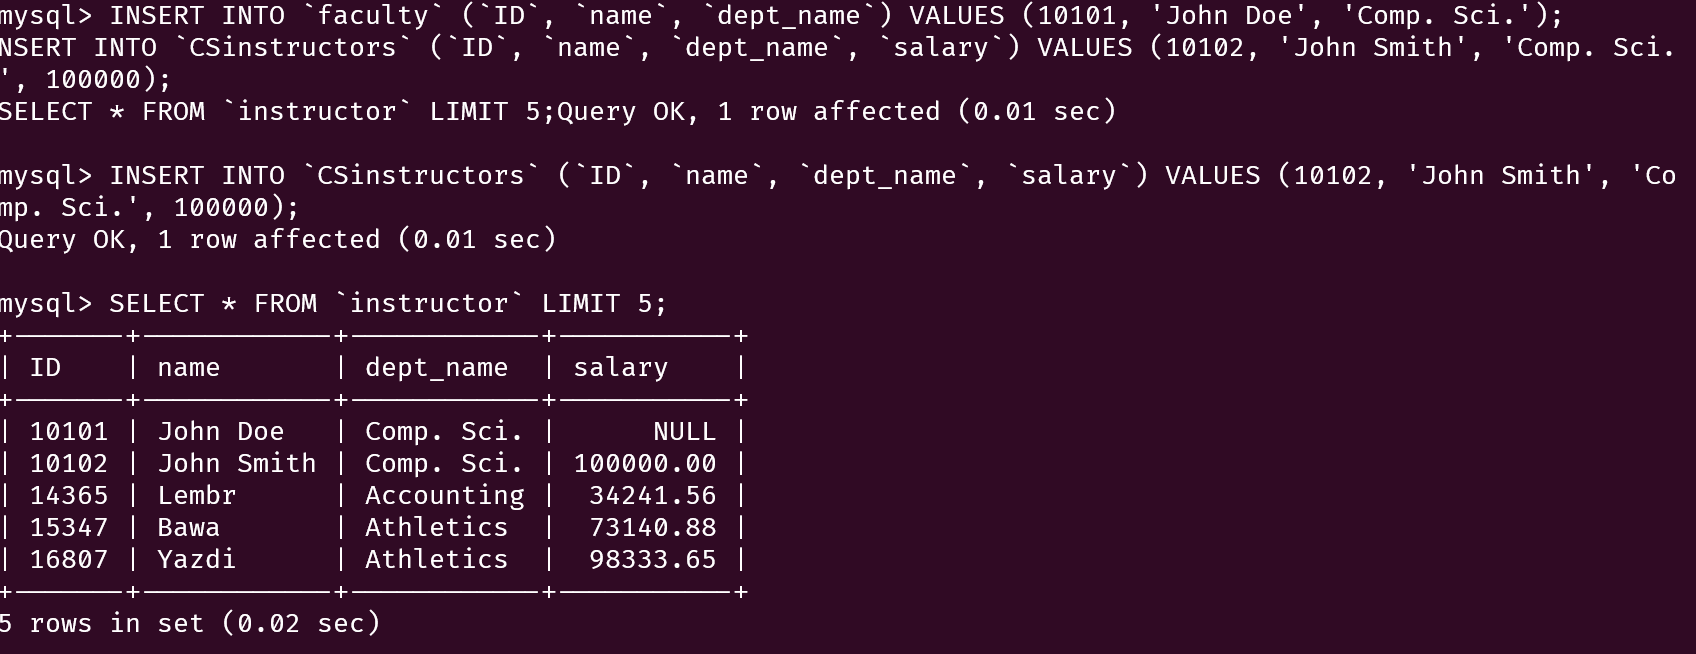
\includegraphics[width=0.9\textwidth]{img/37.png}
\caption{插入数据}
\end{figure}

可以发现原表中的数据也被更新了,说明视图是基于原表的,视图的更新会影响原表。

\item Create a new user and grant permission to the user to view all data in your student relation.

\begin{lstlisting}[language=sql]
create user newuser identified by 'Password@123';
grant select on student to newuser;
-- 切换至newuser用户登录,验证对数据表的权限;
exit;
mysql -unewuser -p -Ddbcourse
select * from advisor;
-- ERROR 1142 (42000): SELECT command denied to user 'newuser'@'localhost' for table 'advisor'
update student set tot_cred = tot_cred + 1;
-- ERROR 1142 (42000): UPDATE command denied to user 'newuser'@'localhost' for table 'student'
select * from student;
-- 切换至root用户登录
exit;
mysql -uroot -p -Ddbcourse
\end{lstlisting}

结果如下:

\begin{figure}[H]
\centering
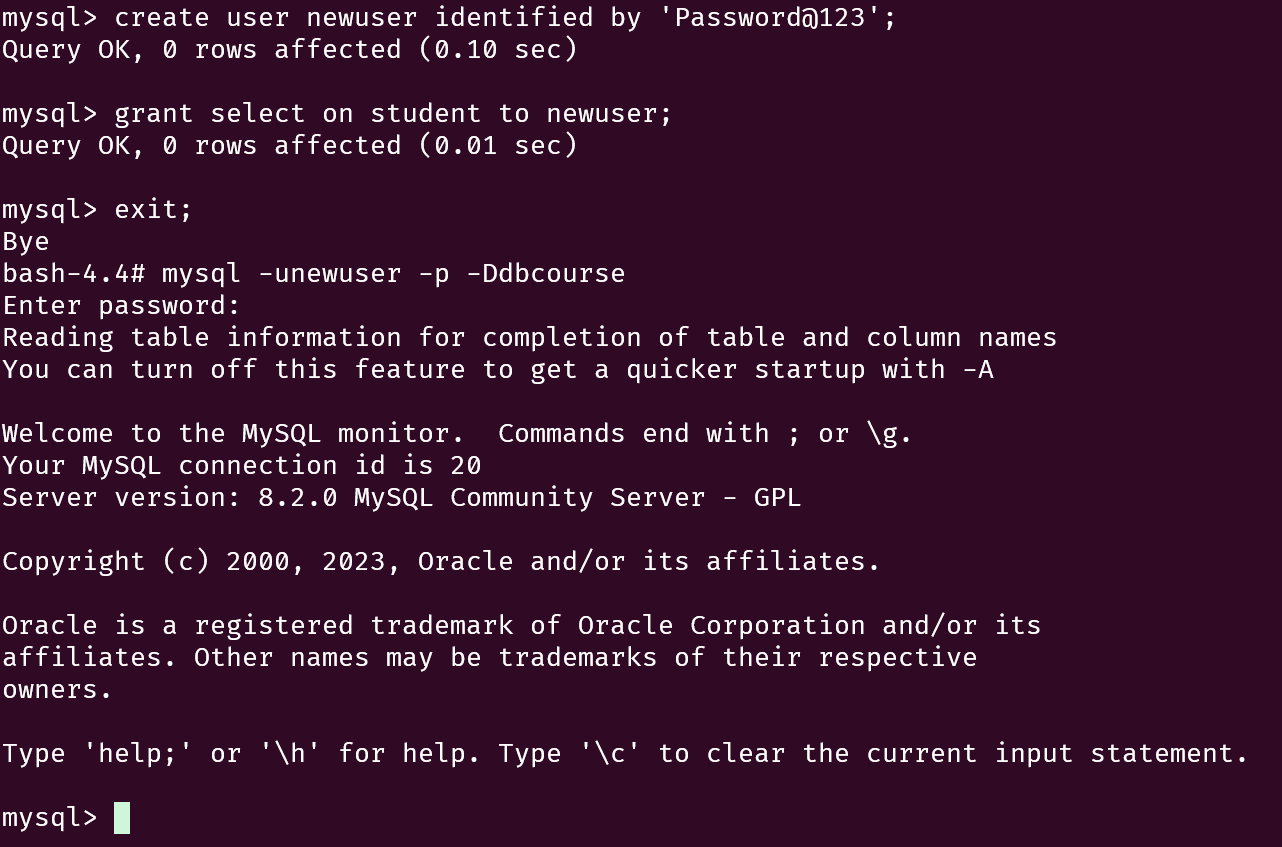
\includegraphics[width=0.9\textwidth]{img/38.png}
\caption{创建用户并授权}
\end{figure}

\begin{figure}[H]
\centering
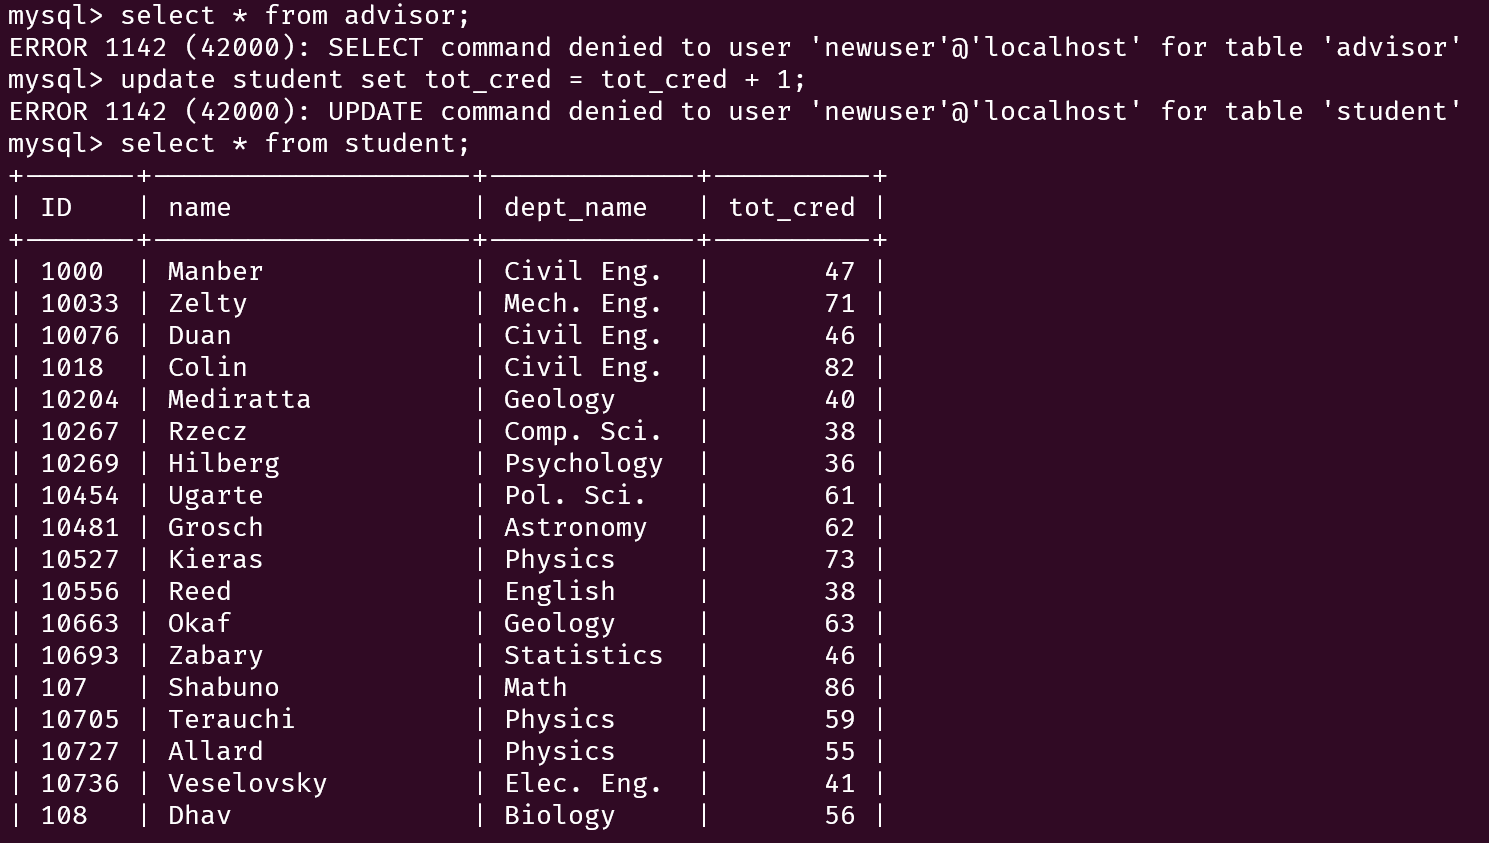
\includegraphics[width=0.7\textwidth]{img/39.png}
\caption{验证用户权限}
\end{figure}

\begin{figure}[H]
\centering
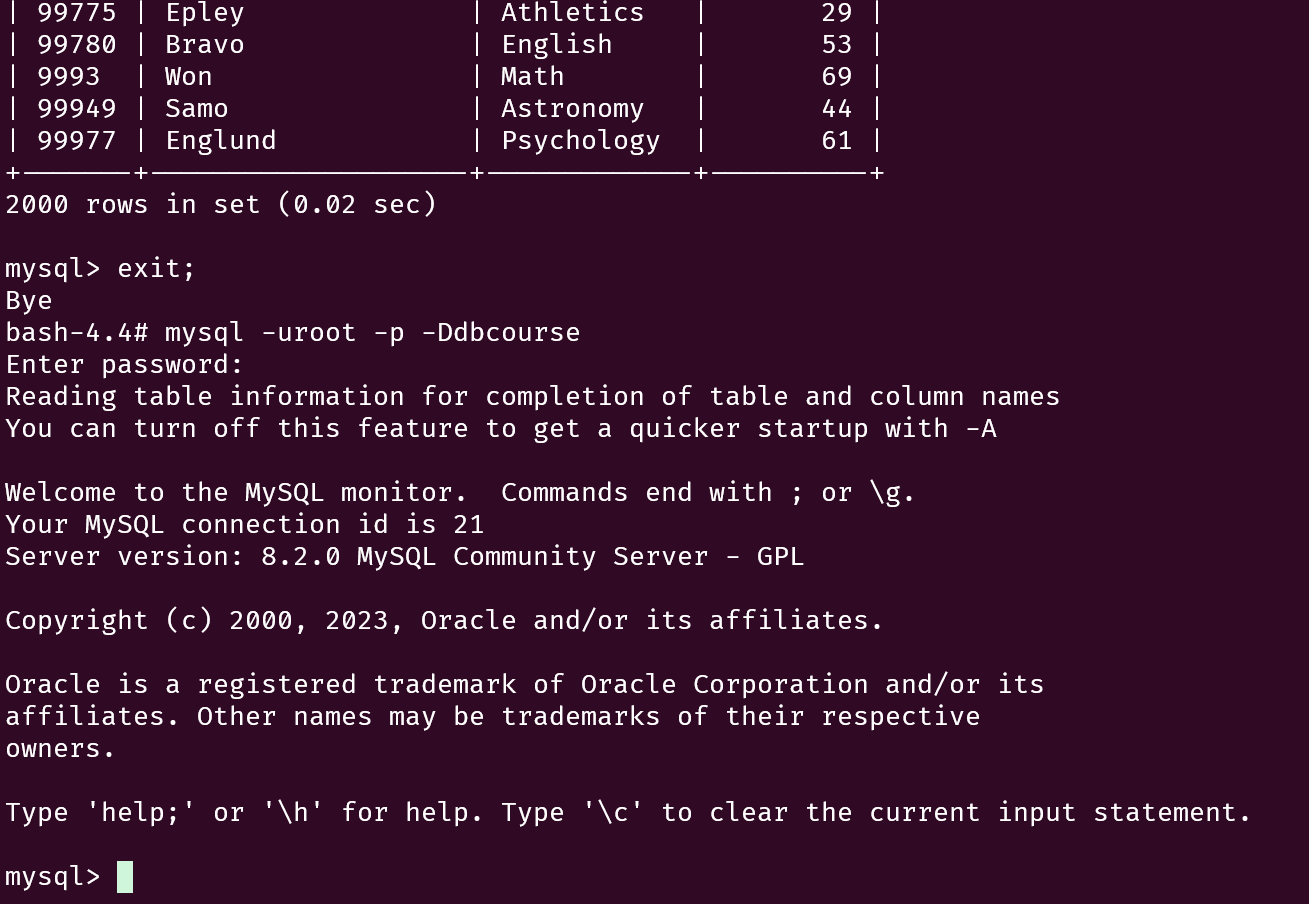
\includegraphics[width=0.7\textwidth]{img/40.png}
\caption{切换用户}
\end{figure}

\item Now grant permission to all users to see all data in your faculty view.

\begin{lstlisting}[language=sql]
create role all_users;
grant all_users to root, newuser;
grant select on faculty to all_users;
-- 切换至newuser用户登录,验证权限
exit;
mysql -unewuser -p -Ddbcourse
set role all_users;
select * from instructor;
select * from faculty;
\end{lstlisting}

结果如下:

\begin{figure}[H]
\centering
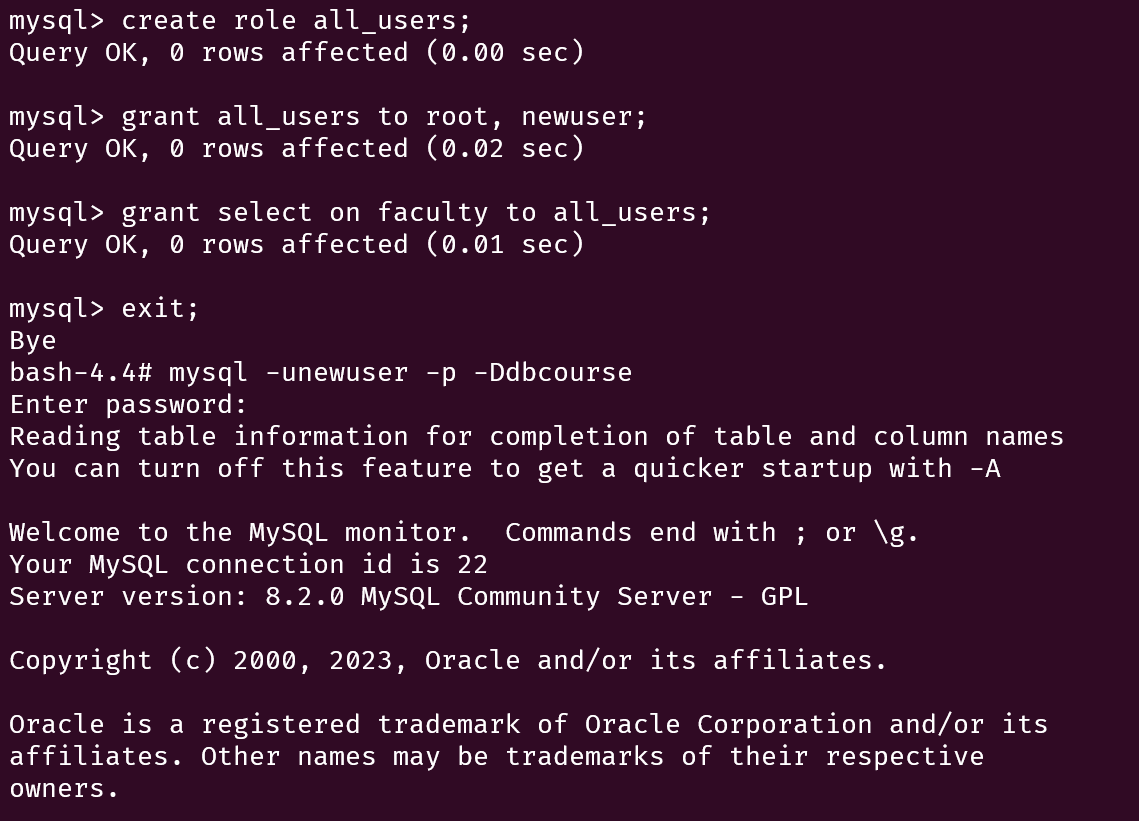
\includegraphics[width=0.9\textwidth]{img/41.png}
\caption{授权用户查看视图}
\end{figure}

\begin{figure}[H]
\centering
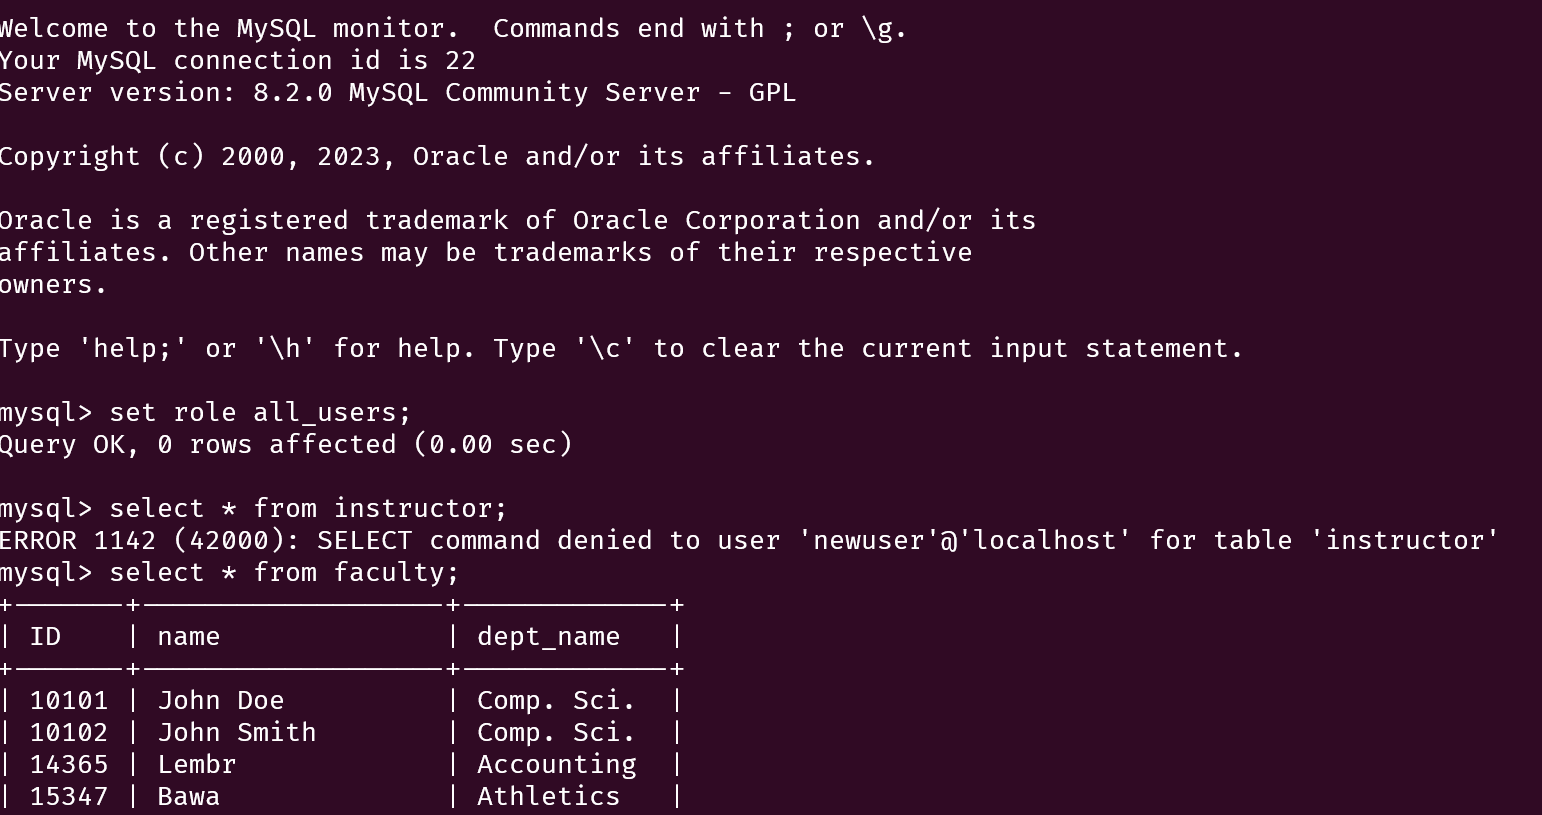
\includegraphics[width=0.9\textwidth]{img/42.png}
\caption{验证用户权限}
\end{figure}

\end{enumerate}

\section{存在的问题及解决方案}

\begin{enumerate}
  \item 对 \texttt{COALESCE} 函数的使用不熟悉,导致在查询中出现错误,通过查阅文档解决了问题。
  \item 更新数据时出现错误,导致数据库内数据被破坏,通过备份数据恢复了数据库。
\end{enumerate}

\section{实验小结}

通过本次实验,我学习了 \texttt{MySQL} 数据库管理系统中\texttt{SQL}的基本语法,掌握了\texttt{SQL}语
句的编写方法,能够编写\texttt{SQL}语句完成指定的查询。同时,我还学习了如何创建数据表、插入数据、创建视图、创建用户、授权用户等操作,对数据库的管理有了更深入的了解。

\end{document}